% !TEX encoding = UTF-8 Unicode
% !TeX TS-program = pdfLaTeX
% !TeX spellcheck = en-US
% !BIB TS-program = bibtex
% -*- coding: UTF-8; -*-
% vim: set fenc=utf-8
%
%%%%%%%%%%%%%%%%%%%%%%%%%%%%%%%%%%%%%%%%%%%%%%%%%%%%%%%%%%%%%%%%%%
%
% public
% https://github.com/SpikeAI/pyTERtorch/ (for dev)
% https://github.com/SpikeAI/2023_GrimaldiPerrinet_HeterogeneousDelaySNN 
% https://www.zotero.org/groups/4776796/fastmotiondetection
%
% private
% https://framateam.org/spikeai/channels/fast-motion-biolcyb
% https://www.overleaf.com/project/630f9044c38e7a3cea81a7b2
%
%%%%%%%%%%%%%%%%%%%%%%%%%%%%%%%%%%%%%%%%%%%%%%%%%%%%%%%%%%%%%%%%%%
%
% Guest Editors:
% 
% Kexin Chen - Department of Cognitive Sciences, University of California, Irvine
% Hirak J. Kashyap - Department of Computer Science, University of California, Irvine
% Jeffrey L. Krichmar - Department of Cognitive Sciences, Department of Computer Science, University of California, Irvine
% Xiumin Li - College of Automation, Chongqing University, Chongqing, China
% 
% Kexin Chen, Hirak Kashyap, Jeffrey Krichmar, Xiumin Li
% NeuroVision Organizing Team
% 
% Kexin Chen <kexinc3@uci.edu>
%
%%%%%%%%%%%%%%%%%%%%%%%%%%%%%%%%%%%%%%%%%%%%%%%%%%%%%%%%%%%%%%%%%%
% 2022-09-30
% Learning heterogeneous delays in a layer of spiking neurons for fast motion detection
% Corresponding Author: Laurent Perrinet
% Biological Cybernetics
% a7f45f8e-87d6-4a30-ac7f-9f0c94e2592a   |  v.1.0
%%%%%%%%%%%%%%%%%%%%%%%%%%%%%%%%%%%%%%%%%%%%%%%%%%%%%%%%%%%%%%%%%%
%%%%%%%%%%%%%%%%%%%%%%%%%%%%%%%%%%%%%%%%%%%%%%%%%%%%%%%%%%%%%%%%%%
%Call for papers: Biological Cybernetics Special Issue: What can Computer Vision learn from Visual Neuroscience?
%
% https://www.springer.com/journal/422/updates/20421374
%
%Computer vision still struggles to solve many problems as quickly and accurately as our brain does, despite its tremendous progress using deep learning over the last decade. Current challenges include geometry understanding, dynamic scene understanding, few shot learning of novel objects, anomaly and counterfeit detection, stable reproduction of imaginary visuals, and more. The brain achieves all these on a low computational cost and power budget (i.e., tens of watts), whereas the state-of-the-art computer vision models require multiple graphics processors consuming kilowatts of power. Hence, new inspirations from the brain could make computer vision more efficient, robust, and capable of continuous learning and adaptation. Although visual neuroscience literature provides knowledge about neuronal selectivities and early processing of visual inputs, computational modelling of neuronal and network behaviours with some degree of biological constraints and characteristics is an important tool to address many of the challenges facing computer vision. With new neuroscientific insights about deep cortical vision processing using the latest stimulation and recording technologies, it is important that we strive to understand the underlying computations and learning mechanisms, so that artificial vision systems with similar efficiency can be developed. This special issue invites original research and review articles related to topics in biological vision that can potentially benefit computer vision systems. The following is a non-exhaustive list of topics in biological vision that can also benefit computer vision systems.
%
%● Active vision’s role in visual search, scene understanding, social interactions, etc.
%
%● Learning in the visual system. Learning in biology is continual, few-shot, and adversarially robust.
%
%● The roles of recurrent and top-down connections in the visual cortex.
%
%● Spike based spatio-temporal processing and its implications for neuromorphic vision.
%
%● Motion perception in dynamic environments.
%
%● Neural coding schemes in the visual system (e.g., sparse coding, predictive coding, and temporal coding.)
%
%● The roles of attention mechanisms in biological vision.
%%%%%%%%%%%%%%%%%%%%%%%%%%%%%%%%%%%%%%%%%%%%%%%%%%%%%%%%%%%%%%%%%%
%%%%%%%%%%%%%%%%%%%%%%%%%%%%%%%%%%%%%%%%%%%%%%%%%%%%%%%%%%%%%%%%%%
\newcommand{\Title}{
Learning heterogeneous delays in a layer of spiking neurons for fast motion detection
}
\newcommand{\ShortTitle}{
Learning heterogeneous delays of spiking neurons for motion detection
}
\newcommand{\FirstAG}{Antoine}
\newcommand{\LastAG}{Grimaldi}
\newcommand{\AuthorAG}{\FirstAG \LastAG}
\newcommand{\FirstLP}{Laurent U}
\newcommand{\LastLP}{Perrinet}
\newcommand{\AuthorLP}{\FirstLP \LastLP}
\newcommand{\EmailLP}{laurent.perrinet@univ-amu.fr}
\newcommand{\EmailAG}{antoine.grimaldi@univ-amu.fr}
\newcommand{\orcidLP}{0000-0002-9536-010X}
\newcommand{\orcidAG}{0000-0002-3107-4788}
\newcommand{\Department}{Institut de Neurosciences de la Timone}% (UMR 7289)}%
\newcommand{\Affiliation}{Aix Marseille Univ, CNRS}%
\newcommand{\Street}{27 boulevard Jean Moulin}%
\newcommand{\PostCode}{13005}%
\newcommand{\City}{Marseille}%
\newcommand{\Country}{France}%
\newcommand{\WebsiteLP}{https://laurentperrinet.github.io}%
\newcommand{\Abstract}{
The response of a biological neuron depends on the precise timing of afferent spikes. This temporal aspect of the neural code is essential to understand information processing in neurobiology and applies particularly well to the output of neuromorphic hardware such as event-based cameras. However, most artificial neural models do not take advantage of this important temporal dimension of the neural code. Inspired by this neuroscientific observation, we develop a model for the efficient detection of temporal spiking motifs based on a layer of spiking neurons with heterogeneous synaptic delays. The model uses the property that the diversity of synaptic delays on the dendritic tree allows for the synchronization of specific arrangements of synaptic inputs as they reach the basal dendritic tree. We show that this can be formalized as a time-invariant logistic regression that can be trained on labeled data. We demonstrate its application to synthetic naturalistic videos transformed into event streams similar to the output of the retina or to event-based cameras and for which we will characterize the accuracy of the model in detecting visual motion. In particular, we quantify how the accuracy can vary as a function of the overall computational load showing it is still efficient at very low workloads. This end-to-end, event-driven computational building block could improve the performance of future spiking neural network (SNN) algorithms and in particular their implementation in neuromorphic chips.
}
\newcommand{\Keywords}{time code, event-based computations, spiking neural networks, motion detection, efficient coding, logistic regression
}
\newcommand{\Funding}{
This research was funded by the European Union ERA-NET CHIST-ERA 2018 research and innovation program under grant agreement N° ANR-19-CHR3-0008-03 (``\href{APROVIS3D}{http://aprovis3d.eu/}''). 
LP received funding from the ANR project  N° ANR-20-CE23-0021 ``\href{AgileNeuroBot}{https://laurentperrinet.github.io/grant/anr-anr/}''
and from A*Midex grant number AMX-21-RID-025
``\href{Polychronies}{https://laurentperrinet.github.io/grant/polychronies/}''. 
}
\newcommand{\Acknowledgments}{
Thanks to % Thomas Schatz, Rosa Cossart,
Hugo Ladret, Camille Besnainou and Jean-Nicolas Jérémie for useful discussions prior to the elaboration of this work. 
\Funding %
%For the purpose of open access, the author has applied a CC BY public copyright licence to any Author Accepted Manuscript version arising from this submission. This research was funded, in whole or in part, by [Organisation name, Grant #]. 
A CC-BY public copyright license has been applied by the authors to the present document and will be applied to all subsequent versions up to the Author Accepted Manuscript arising from this submission, in accordance with the grant’s open access conditions. 
}
\newcommand{\DataAvailability}{
This works is made reproducible. The code reproducing the manuscript and all figures is available on~\href{ https://github.com/SpikeAI/2023_GrimaldiPerrinet_HeterogeneousDelaySNN}{GitHub}. It also contains supplementary figures and results. Find also the associated~\href{https://www.zotero.org/groups/4776796/fastmotiondetection}{zotero group} used to gather relevant literature on the subject.
}
%%%%%%%%%%%%%%%%%%%%%%%%%%%%%%%%%%%%%%%%%%%%%%%%%%%%%%%%%%%%%%%%%%%%%

%%%%%%%%%%%%%%%%%%%%%%%%%%%%%%%%%%%%%%%%%%%%%%%%%%%%%%%%%%%%%%%%%%%%%
%%                                                                 %%
%% Please do not use \input{...} to include other tex files.       %%
%% Submit your LaTeX manuscript as one .tex document.              %%
%%                                                                 %%
%% All additional figures and files should be attached             %%
%% separately and not embedded in the \TeX\ document itself.       %%
%%                                                                 %%
%%%%%%%%%%%%%%%%%%%%%%%%%%%%%%%%%%%%%%%%%%%%%%%%%%%%%%%%%%%%%%%%%%%%%

%%\documentclass[referee,sn-basic]{sn-jnl}% referee option is meant for double line spacing

%%=======================================================%%
%% to print line numbers in the margin use lineno option %%
%%=======================================================%%

%%\documentclass[lineno,sn-basic]{sn-jnl}% Basic Springer Nature Reference Style/Chemistry Reference Style

%%======================================================%%
%% to compile with pdflatex/xelatex use pdflatex option %%
%%======================================================%%

%%\documentclass[pdflatex,sn-basic]{sn-jnl}% Basic Springer Nature Reference Style/Chemistry Reference Style

%%\documentclass[sn-basic]{sn-jnl}% Basic Springer Nature Reference Style/Chemistry Reference Style
%%\documentclass[sn-mathphys]{sn-jnl}% Math and Physical Sciences Reference Style
%%\documentclass[sn-aps]{sn-jnl}% American Physical Society (APS) Reference Style
%%\documentclass[sn-vancouver]{sn-jnl}% Vancouver Reference Style
%%\documentclass[sn-apa]{sn-jnl}% APA Reference Style
%%\documentclass[sn-chicago]{sn-jnl}% Chicago-based Humanities Reference Style
%%\documentclass[sn-standardnature]{sn-jnl}% Standard Nature Portfolio Reference Style
\documentclass[default]{sn-jnl}% Default
%%\documentclass[default,iicol]{sn-jnl}% Default with double column layout
%%\documentclass[iicol]{sn-jnl}

\usepackage[T1]{fontenc}
%\usepackage{textcomp}
\usepackage[utf8]{inputenc}
%
\usepackage{lineno}
\linenumbers

%%%% Standard Packages
%%<additional latex packages if required can be included here>
%\usepackage[lofdepth,lotdepth,position=top]{subfig}
%\usepackage{tabularx}
%%%%

%%%%%=============================================================================%%%%
%%%%  Remarks: This template is provided to aid authors with the preparation
%%%%  of original research articles intended for submission to journals published 
%%%%  by Springer Nature. The guidance has been prepared in partnership with 
%%%%  production teams to conform to Springer Nature technical requirements. 
%%%%  Editorial and presentation requirements differ among journal portfolios and 
%%%%  research disciplines. You may find sections in this template are irrelevant 
%%%%  to your work and are empowered to omit any such section if allowed by the 
%%%%  journal you intend to submit to. The submission guidelines and policies 
%%%%  of the journal take precedence. A detailed User Manual is available in the 
%%%%  template package for technical guidance.
%%%%%=============================================================================%%%%

\jyear{2023}%
%% as per the requirement new theorem styles can be included as shown below
\theoremstyle{thmstyleone}%
\newtheorem{theorem}{Theorem}%  meant for continuous numbers
\newtheorem{proposition}[theorem]{Proposition}% 
%
\theoremstyle{thmstyletwo}%
\newtheorem{example}{Example}%
\newtheorem{remark}{Remark}%

\theoremstyle{thmstylethree}%
\newtheorem{definition}{Definition}%

\raggedbottom

\newcommand{\seeFig}[1]{see Fig.~\ref{fig:#1}}%{see Figure~\ref{fig:#1}}
%% The preceding line is only needed to identify funding in the first footnote. If that is unneeded, please comment it out.
%\usepackage{cite}
%\usepackage[usenames,dvipsnames]{xcolor} %The package starts from the basic facilities of the color package, and provides easy driver-independent access to several kinds of color tints, shades, tones, and mixes of arbitrary colors.
%\usepackage{tcolorbox} % define boxes that can be customed, has to be loaded after xcolor package
\usepackage{amsmath,amssymb,amsfonts} % amsmath and amssymb packages, useful for mathematical formulas and symbols
%%\usepackage{float} %allows me to use [H] with figures to insert figures in multicol env (poster)
%\usepackage{ulem} %The package provides an \ul (underline) command which will break over line ends; this technique may be used to replace \em (both in that form and as the \emph command), so as to make output look as if it comes from a typewrite. Caution: with this package, bibliography will make unbreakable and underlined journal titles
%\usepackage[switch]{lineno} % add line numbers
%\modulolinenumbers[5]
\usepackage{physics} %The  goal  of  this  package  is  to  make  typesetting  equations  for  physics  simpler,  faster,  and  more  human-readable.
%\usepackage{hyperref} %The hyperref package is used to handle cross-referencing commands in LaTeX to produce hypertext links in the document
%\hypersetup{
%    colorlinks = false,
%    hidelinks
%    %linkbordercolor = {white},
%}
%\usepackage{array} %An extended implementation of the array and tabular environments which extends the options for column formats, and provides “programmable” format specifications.
%\usepackage{multicol} %Multicol defines a multicols environment which typesets text in multiple columns
%%\usepackage{wrapfig} %Allows figures or tables to have text wrapped around them. wrapfig is used when calling multicols
% \usepackage[position=top]{subfig} %The package provides support for the manipulation and reference of small or ‘sub’ figures and tables within a single figure or table environment. Linked to subfloat.
% for units
\usepackage{siunitx}%The siunitx package provides a  set  of  tools  for  authors  to  typeset  quantities  in  aconsistent  way.
%\AtBeginDocument{\RenewCommandCopy\qty\SI}
\DeclareMathOperator*{\argmax}{arg\,max}
\DeclareMathOperator*{\argmin}{arg\,min}
%%%%%%%%%%%%%%%%%%%%%%%%%%%%%%%%%%%%%%%%%%%%%%%%%%%%%%%%%%%%%%%%%%%%%
% NOTATIONS
\newcommand{\ms}{\si{\milli\second}}%
\newcommand{\us}{\si{\micro\second}}%
\newcommand{\presynaddr}{a} % pre address
\newcommand{\postsynaddr}{b} % post address
\newcommand{\numevent}{N_{ev}} % total number of events
\newcommand{\presynaddrspace}{\mathcal{A}} %presynaptic address space
\newcommand{\postsynaddrspace}{\mathcal{B}} %postsynaptic address space
\newcommand{\Npol}{N_\text{p}} % number of polarity
\newcommand{\Nneuron}{N_\text{n}} % number of output neurons in the layer
\newcommand{\arank}{r} % address index
\newcommand{\bias}{\beta} % bias for the MLR model
\newcommand{\synapse}{\mathcal{S}} % synapse
\newcommand{\synapticweight}{w} % synaptic weight
\newcommand{\synapticdelay}{\delta} % synaptic delay
\newcommand{\ranksyn}{s} % synapse index
\newcommand{\Nsyn}{N_{s}} % total number of synapses
\newcommand{\activeweights}{\mathcal{W}} 
\newcommand{\timev}{t} % time
\newcommand{\polev}{p} % polarity
\newcommand{\event}{\epsilon} % event
\newcommand{\eventstream}{\xi} % stream of events
\newcommand{\TS}{S} % time surface
\newcommand{\neuron}{\mathbf{n}} % neuron in the SNN (defined by the spatial position and the channel)
\newcommand{\postneuron}{\mathbf{m}} % post synaptic neuron in the SNN (defined by the spatial position and the kernel)
\newcommand{\channel}{\mathbf{p}} % channel
\newcommand{\layer}{\mathbf{L}} % layer
% \newcommand{\timecontext}{T} % time context (cf HOTS) matrice gathering last event times
\newcommand{\current}{I} % post synaptic current
\newcommand{\volt}{u} % membrane potential
\newcommand{\volts}{V} % matrix of membrane potentials
\newcommand{\gain}{\gamma} % homeostatic gain
% \newcommand{\simil}{\beta} % similarity value
\newcommand{\Nclass}{N_\text{class}} % number of classes for MLR:
\newcommand{\Nx}{N_\text{X}}
\newcommand{\Ny}{N_\text{Y}}
\newcommand{\Ntime}{N_\text{T}}
\newcommand{\kernel}{\mathcal{K}} % convolution kernel
%\newcommand{\kernelind}{\mathbf{k}} % indice of the kernel
\newcommand{\kernelind}{k} % indice of the kernel
\newcommand{\Kx}{K_\text{X}}
\newcommand{\Ky}{K_\text{Y}}
\newcommand{\Ktime}{K_\text{T}}
\newcommand{\classiflayer}{\mathbf{C}}
\newcommand{\class}{c} % class k of the MLR
\newcommand{\lrweights}{\theta} % matrix of MLR weights
\newcommand{\lrtrue}{y} % true value of the prediction for MLR
\newcommand{\loss}{J} % cost function for MLR
\newcommand{\softmax}{\sigma}
\newcommand{\actfreq}{f}
\newcommand{\decision}{\hat{y}}
\newcommand{\colorsec}{black}
\newcommand{\colorsubsec}{black}
\newcommand{\speed}{v}
\newcommand{\Nspeed}{N_v}
% Example definitions.
% --------------------
\def\x{{\mathbf x}}
\def\L{{\cal L}}
%%%%%%%%%%%%%%%%%%%%%%%%%%%%%%%%%%%%%%%%%%%%%%%%%%%%%%%%%%%%%%%%%%
%%%%%%%%%%%%%%%%%%%%%%%%%%%%%%%%%%%%%%%%%%%%%%%%%%%%%%%%%%%%%%%%%%
% a simpler annotation system:
\usepackage{soulutf8}
\usepackage{color}
\newcommand{\note}[1]{{\sethlcolor{yellow}\hl{#1}}}
%\newcommand{\note}[1]{}
%
\begin{document}
%%%-----------------------------------------------------------------
\title[\ShortTitle]{\Title}
\artnote{This article is published as part of the Special Issue on "What can Computer Vision learn from Visual Neuroscience?"}
% ---------------
\author{\fnm{\FirstAG} \sur{\LastAG}}\email{\EmailAG}
\author{\fnm{\FirstLP} \sur{\LastLP}}\email{\EmailLP}
\affil{\orgdiv{\Department}, \orgname{\Affiliation}\\ \orgaddress{\street{\Street}, \city{\City}, \postcode{\PostCode}, \country{\Country}}}
%
\abstract{
\Abstract
}

\keywords{\Keywords}
%
\maketitle
%
\section{Introduction}
%%%-----------------------------------------------------------------
\label{sec:intro}
%
The human brain has the remarkable property of being able to react at any time while consuming a reasonable amount of energy, about tens of watts. This system is the result of millions of years of natural selection, and a striking difference with artificial neural networks is the representation both use. Artificial convolutional neural networks (CNNs), for example, represent the flow of information from one layer to another as tensors, storing visual information densely across the visual topography, with different properties represented in different channels. These networks are known to mimic many properties of biological systems, such that each can be attributed a ``Brain Score''~\citep{schrimpf_brain-score_2020}, yet this score takes no account of inference speed or energy consumption. CNNs have achieved state-of-the-art performance for some computer vision tasks, such as image recognition. However, they do not take advantage of the dynamics inherent in the way we perceive our natural environment. In the vast majority of biological neural networks, on the other hand, information is represented as \emph{spikes}, prototypical all-or-nothing events whose only parameters are their timing and the address of the neuron that fired the spike~\citep{paugam-moisy_computing_2012}. The third generation of artificial neural networks, known as spiking neural networks (SNNs), incorporates this temporal dimension into the way they perform their computations. They are of interest for computational neuroscience because they provide a better model of the biological neuron. Some approaches have developed normative models of SNNs that aim to have applications in machine learning. One of these is the SpikeNet algorithm, which uses a purely temporal approach by encoding information using one spike per neuron~\citep{delorme_spikenet_1999}. Another type of SNN that uses accurate timing of spikes attempts to determine the structure of the network to minimize a cost function. This was implemented in the SpikeProp algorithm~\citep{bohte_error-backpropagation_2002} and has been recently extended. This method uses a surrogate gradient and is now widely used in attempts to transfer the performance of CNNs to SNNs~\citep{zenke_remarkable_2021}. However, the performance of SNNs still lags behind that of firing-rate based networks. The question of the advantage of using spikes in machine learning and computer vision remains open.

In a recent review paper, we reported experimental evidence for the presence of precise spiking motifs embedded in recordings from biological neural tissues~\cite{grimaldi_precise_2023}. These spatio-temporal motifs within the neural activity may be useful representations to perform computations for various cognitive tasks. Notably, \citet{abeles_role_1982} asked whether the role of cortical neurons is the integration of synaptic inputs or rather the detection of coincidences in temporal spiking motifs. While the first possibility favors the firing-rate coding theory, the second one emphasizes the function of temporal precision in the neural code. Since then, numerous studies have demonstrated the emergence of synchronicity of activity within a neuronal population~\citep{riehle_spike_1997, davis_spontaneous_2021}, efficient coding using spike latencies~\citep{perrinet_coding_2004, gollisch_rapid_2008} or precise timing in the auditory system~\citep{deweese_binary_2002, carr_circuit_1990}. All these findings, and more~\citep{bohte_evidence_2004}, highlight the importance of the temporal aspect of the neural code and suggest the existence of spatio-temporal spiking motifs in biological spike trains. In neural models, the integration of heterogeneous delays~\citep{guise_bayesian_2014, zhang_supervised_2020, nadafian_bio-plausible_2020} allows for the efficient exploitation or detection of these spatio-temporal motifs embedded in the spike train. In particular,~\citet{izhikevich_polychronization_2006} introduced the notion of the polychronous group as a repetitive motif of spikes defined by a subset of neurons with different, but precise, relative spiking delays, i.e., the time between the arrival of an afferent spike at a given synapse and the contribution of the associated postsynaptic potential to the neuron's soma. Due to the variety of configurations and the possible coexistence of multiple superimposed motifs, representation with polychronous groups has a much higher information capacity than a firing rate-based approach to neural coding.

The present paper proposes additional experiments extending a recent model of spiking neurons with heterogeneous synaptic delays~\cite{grimaldi_learning_2022}. This model was trained to solve a motion detection task on a synthetic event-based dataset generated by moving parameterized textures. Once trained, the volume of event-driven computations could be drastically reduced by pruning the synapses, while maintaining top performance for the classification task. This was a demonstration that formal neurons can exploit the precise timing of spikes to improve neural computations. In the present work, we extend motion detection to a more ecological task. Instead of the synthetic textures that have been used to generate motion-driven stimuli, we use natural images and random movements that mimic biological saccades. Using an ecological motion detection task, we study the emergence of spatio-temporal spiking motifs when a single layer of spiking neurons is trained on a supervised classification task. First, we define the ecological cognitive task the model has to solve with the different datasets it will be tested on. Then, we develop a theoretically defined Heterogeneous Delays Spiking Neural Network (HD-SNN) model capable of learning these heterogeneous synaptic delays. We will investigate the efficiency of the motion detection mechanism and in particular its resilience to synaptic weight pruning. In this way, we will be able to show how such a model can provide an efficient solution to the trade-off between energy and accuracy.
%
%%%-----------------------------------------------------------------
%%%-----------------------------------------------------------------
\section{Methods}
\label{sec:methods}
%%%-----------------------------------------------------------------
In this paper, we aim to test whether the HD-SNN model is capable of efficiently learning a motion detection task, which is defined by a realistic event-based data stream. This type of signal is typically captured by a Dynamic Vision Sensor (DVS) and is inspired by the signal that is sent from the retinal ganglion cells through the optic nerve. The events are binary in nature and should be sufficient to perform the task of motion detection in a fast and efficient manner. Here we will first describe the task definition and then the HD-SNN model we use for motion inference and how we train it. 
%%%-----------------------------------------------------------------
%
\subsection{Task definition: motion detection in a synthetic naturalistic event stream}\label{sec:task}
%%%-----------------------------------------------------------------
To train and test our model, we need to define a visual dataset for which we control the direction and speed of motion. Let us now define a procedure for animating a natural visual scene with virtual eye movements, similar to those used in neurobiological~\citep{vinje_sparse_2000, baudot_animation_2013} and computational neuroscience~\citep{kremkow_push-pull_2016} studies. First, we draw a trajectory inspired by the biological movements of the eyes. Indeed, these movements allow us to dynamically actuate the center of vision, or gaze, in the visual field. In animals with a fovea, this is particularly useful because it allows the area with the highest density of photoreceptors in the environment to be moved, for example to a point of interest. A specific mechanism for this function are saccades, which are rapid eye movements that reposition the center of vision. In humans, saccades are very frequent (on average $2$ per second~\citep{dandekar_neural_2012}). They are generated very quickly (about $80~\ms$) and have a wide range of speeds. On a more microscopic scale, the human gaze moves with a continuous drift similar to a Brownian trajectory~\citep{poletti_head-eye_2015}. In order to maintain the full generality of the task, we will define eye movements using a form of random walk~\citep{engbert_integrated_2011}. This approach first defines a finite set of possible 2D movements in polar coordinates. Based on the distribution of biological movements, we simplified it by selecting a set of eye movements as the Cartesian product of $8$ linearly spaced movement directions and 3 geometrically spaced speeds. Next, we define a gaze trajectory as segments whose duration is drawn from a Poisson distribution with a mean block length of $24~\ms$, similar to a Lévy flight~\citep[p. 289]{mandelbrot_fractal_1982}. Finally, the trajectory is integrated, assuming first that the velocities are sampled uniformly and independently from the set of different motion sets, and second that the motion is uniform during a time segment. The resulting instances yield trajectories that are qualitatively similar to those observed for human eye movements (\seeFig{motion_task}-\textit{(Left)}).

%%%-----------------------------------------------------------------
%: fig:motion_task
%%%-----------------------------------------------------------------
\begin{figure}%[h!]%[ht!]
    \centering
    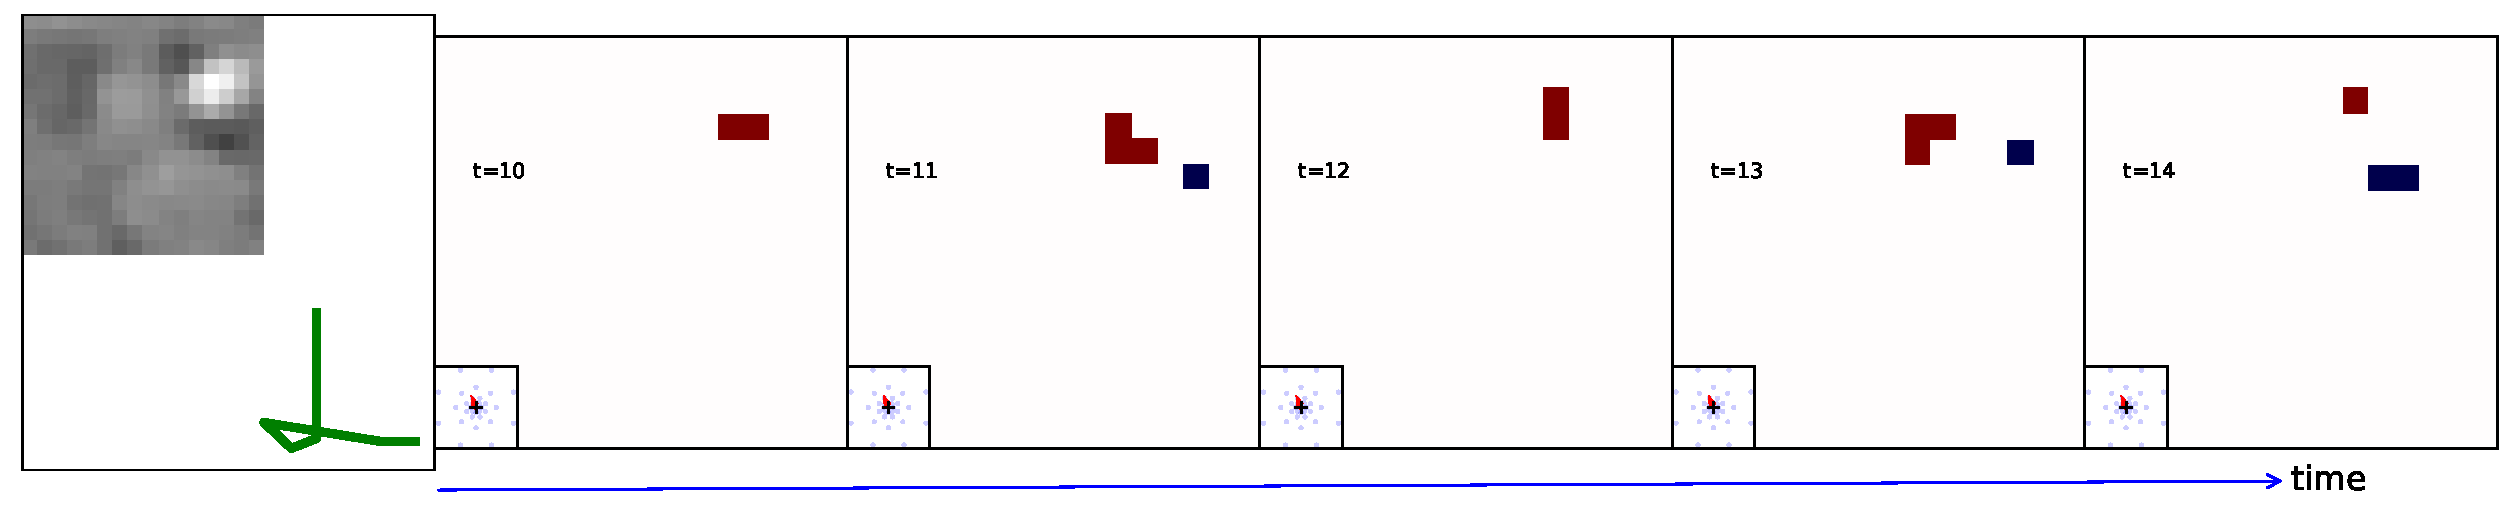
\includegraphics[width=0.95\linewidth]{figures/motion_task.pdf}
    \caption{
        {\bf - Motion Detection Task.} \textit{(Left)}~We use large natural images ($256\times256$) in which an aperture ($64\times64$) extracts a cropped image around the view axis. To mimic the effect of a saccadic eye movement, the view axis moves according to a stepwise random walk. We show such a trajectory with a length of $128$ time steps (green line). \textit{(Right)}~Snapshots of the synthetic event stream at different time steps (start and end frames marked by a white and black dot, respectively). The dynamics of the cropped image translated according to the trajectory as a function of time produces a naturalistic movie, which is then transformed into an event-based representation. Mimicking the retina, this representation encodes proportional increases or decreases in luminance, i.e. ON (red) and OFF (blue) events, in each pixel of the image. In the lower left corner of the snapshots, the translation vector is shown in red as one of the possible classes of motion. Note the change in the direction of motion between the third and fourth image, and also that, due to the aperture problem, contours parallel to the motion emit relatively fewer spikes.}
    \label{fig:motion_task}
\end{figure}
%%%-----------------------------------------------------------------
Once these eye trajectories are generated, we can apply them to a visual scene.  
For this purpose, we selected a database of $600$ natural images that were previously used to study the statistics of natural images~\citep{perrinet_edge_2015}. Note that these have been pre-processed to be in grayscale and to equalize (i.e., whiten) the energy in each frequency band. This process is known to occur in the retino-thalamic pathway~\citep{dan_efficient_1996}. These images are $256 \times 256$ in size, and we will extract sub-images of size $64 \times 64$ positioned around the center of gaze at each time step. We will discretize time in $1~\ms$ bins and produce movies of duration $N_T = 128~\ms$. To avoid boundary effects, we will randomly position the full trajectory in image space such that the subimage is translated using the position given by the trajectory at each time step without touching the borders. At each point in time, the translation is computed using a coordinate roll in the horizontal and vertical dimensions, followed by a sub-pixel translation defined in Fourier space~\citep{perrinet_sparse_2015}. Note that the magnitude of the displacement is relative to the time bin, and we have defined the unit velocity to correspond to a movement of one pixel per frame (i.e., per time bin).

To transform each movie into events as the ones recorded by a DVS, we compute a gradient image (initialized at zero) by computing the temporal gradient of the pixels' intensity over two successive frames. For a specific pixel and timestamp, an event is generated if the absolute value of this gradient exceeds a threshold. The event has either an OFF or ON polarity respectively, whether the gradient is negative or positive. This signed threshold value is then subtracted from the residual gradient image. When applied to the whole movie, the event stream is similar to the output of a neuromorphic camera~\citep{rasetto_challenges_2022}, that is, a list of events defined by $x_\arank$ and $y_\arank$ (their position on the pixel grid), their polarity $\polev_\arank$ (ON or OFF) and time $\timev_\arank$  (\seeFig{motion_task}-\textit{(Right)}). The goal here is to infer the correct motion solely by observing these events. 
% \note{ the task is full-field rigid translations, the model resolves it locally (analogy to the input from V1 to MT) }
%%%-----------------------------------------------------------------
\subsection{The Heterogeneous Delays SNN (HD-SNN) model}
%----------------------------%
%
\begin{figure}%[t!]
    \centering
    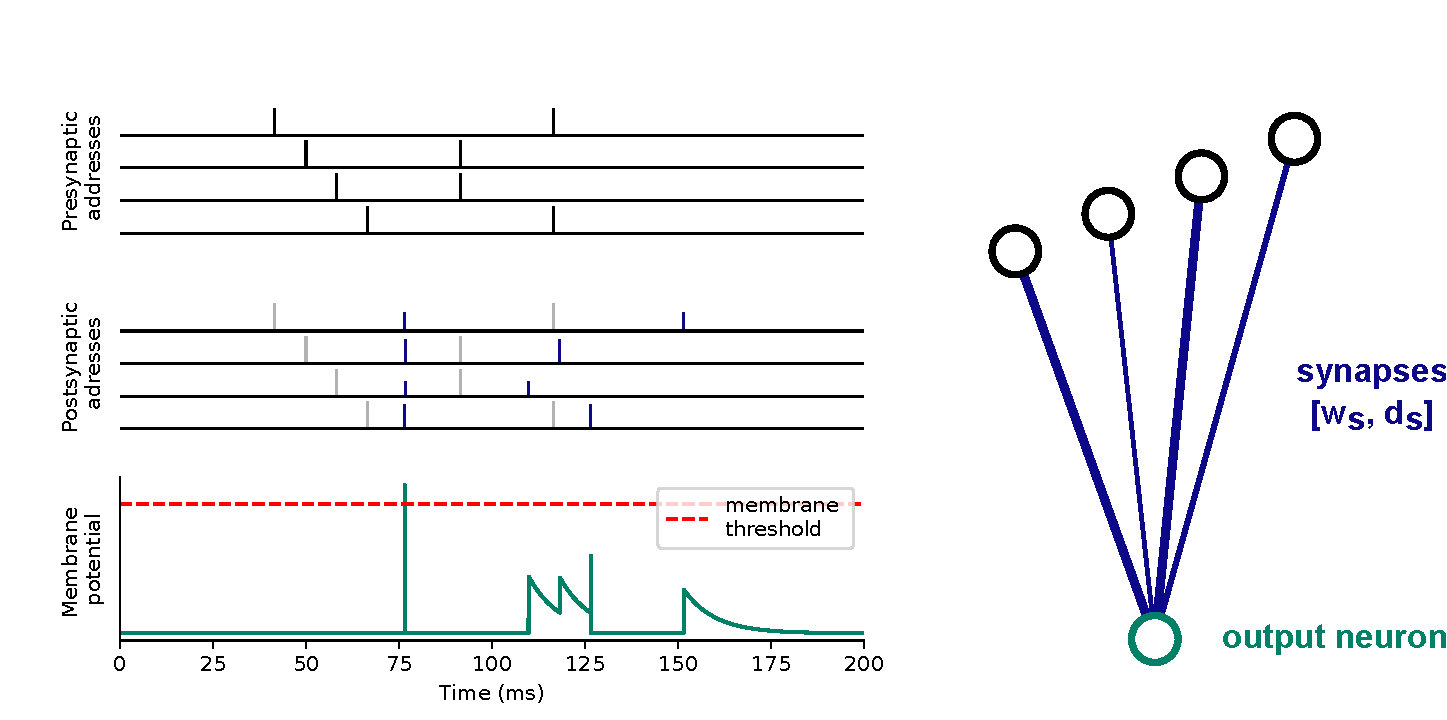
\includegraphics[width=0.980\linewidth]{figures/HDSNN_graph.pdf}
    \caption{\textbf{The core mechanism of the HD SNN model.} \textit{(Top-Left)}~Two spiking motifs are emitted from four presynaptic neurons. Once integrated by the synapses of the postsynaptic neuron~\textit{(Right)}, the spiking motifs are shifted in time by the synaptic delays and weighted by the synaptic weights~\textit{(Middle-Left)}. When they reach the soma of the postsynaptic neuron, the different spikes contribute to a modification of its membrane potential according to an activation function. In this example we use the same activation function as for a Leaky Integrate and Fire neuron~\textit{(Bottom-Left)}. The first spiking motif is synchronized by the synaptic delays and causes a sudden rise in the membrane potential of the postsynaptic neuron. An output spike is emitted when the membrane potential reaches the threshold and it is then reset.   \textit{(Right)}~An illustration of a spiking neuron with different synaptic weights (represented by the thickness of the synapses) and different synaptic delays (represented by the length of the synapses). }%
    \label{fig:izhikevich}%
\end{figure}%
% 
%----------------------------%
In a neurobiological recording or in the sensory signal obtained from an event-based camera, the input consists of a stream of \emph{spikes} or \emph{events}. This can be formalized as a list of neural addresses and timestamps tuples $\event = \{(\presynaddr_\arank, \timev_\arank)\}_{\arank \in [1,\numevent]}$ where $\numevent \in \mathbb{N} $ is the total number of events in the data stream and the rank $\arank$ is the index of each event in the list of events (\seeFig{izhikevich}-\textit{(Top-Left} for an illustration). Events are typically ordered by their time of occurrence. Each event has a time of occurrence $\timev_\arank$ and an associated address $\presynaddr_\arank$. This defines an address space $\presynaddrspace$ which consists of the set of possible addresses. In a neurobiological recording, this can be the identified set of presynaptic neurons. For neuromorphic hardware, this can be defined as $[1, \Npol] \times [1, \Nx]\times[1, \Ny] \subset \mathbb{N}^3$ where $\Npol$ is the number of polarities ($\Npol=2$ for the ON and OFF polarities coded in event-based cameras) and $(\Nx, \Ny)$ is the height and width of the image in pixels. As such, an address $\presynaddr_\arank$ is typically in the form $(\polev_\arank, x_\arank, y_\arank)$ for event-based cameras.

In the HD-SNN model, each neuron $\postsynaddr \in \postsynaddrspace$ connects to presynaptic afferent neurons from $\presynaddrspace$. In biology, a single cortical neuron has generally several thousands of synapses. Each synapse may be defined by its synaptic weight and its delay, that is, the time it takes for one spike to travel from the presynaptic neuron's soma to that of the postsynaptic neuron. A postsynaptic neuron $\postsynaddr \in \postsynaddrspace$ is then described by the synaptic weights connecting it to a presynaptic afferent from $\presynaddrspace$ but also by the set of possible delays. Note that a neuron may contact the same afferent neuron with different delays through different synaptic connections. Scanning all neurons $\postsynaddr$, we thus define the full set of $\Nsyn$ synapses, 
as $\synapse = \{(\presynaddr_\ranksyn, \postsynaddr_\ranksyn, \synapticweight_\ranksyn, \synapticdelay_\ranksyn)\}_{\ranksyn \in [1,\Nsyn]}$, where each synapse is associated to a presynaptic address $\presynaddr_\ranksyn$, a postsynaptic address $\postsynaddr_\ranksyn$, a weight $\synapticweight_\ranksyn$, and a delay $\synapticdelay_\ranksyn$. This defines the full connectivity of the HD-SNN model (\seeFig{izhikevich}-\textit{(Right)} for an illustration of the connectivity of one neuron with synaptic weights and delays). 

Of interest is to define the receptive field of a postsynaptic neuron $\synapse^\postsynaddr =  \{(\presynaddr_\ranksyn, \postsynaddr_\ranksyn, \synapticweight_\ranksyn, \synapticdelay_\ranksyn) \| \postsynaddr_\ranksyn=\postsynaddr\}_{\ranksyn \in [1,\Nsyn]}  \subset \synapse$, or the emitting field of a presynaptic neuron $\synapse_\presynaddr = \{(\presynaddr_\ranksyn, \postsynaddr_\ranksyn, \synapticweight_\ranksyn, \synapticdelay_\ranksyn) \| \presynaddr_\ranksyn=\presynaddr\}_{\ranksyn \in [1,\Nsyn]} \subset \synapse$. As a consequence, a postsynaptic neuron $\postsynaddr$ receives an event stream which is multiplexed by the synapses of its receptive field. It results in a weighted event stream (\seeFig{izhikevich}-\textit{(Middle-Left}) for each  postsynaptic neuron $\postsynaddr$: 
%
\begin{linenomath*}
\begin{equation}\label{eq:stream_b}
\event_\postsynaddr = \{(\presynaddr_\arank, \synapticweight_\arank, \timev_\arank+\synapticdelay_\ranksyn) \| \presynaddr_\arank = \presynaddr_\ranksyn \}_{\arank \in [1,\numevent], \ranksyn \in \synapse^\postsynaddr}
\end{equation}
\end{linenomath*}
%
In biology, this new stream of events is naturally ordered in time as events reach the soma of postsynaptic neurons. However, it should be properly reordered in simulations. Crucially, when postsynaptic neurons are activated on their soma by a specific spatio-temporal motif which is imprinted in the set of synapses, the discharge probability will increase, notably when these spikes converge on the soma in a synchronous manner while the activation function of the neurons of the HD-SNN can be selected among the whole range of spiking neuron response functions (\seeFig{izhikevich}). We defined the HD-SNN model in this subsection in all generality, and in the next subsection, we describe an implementation of our model adapted for the motion detection task. 
%
\subsection{Application of the HD-SNN model to the motion detection task}
%
It is possible to define a specific implementation of this model in order to adapt it to common tasks in computer vision. In particular, from the perspective of simulating such event-based computations on standard CPU- or GPU-based computers and then using parallel computing, it is useful to transform this event-based representation into a dense representation. Indeed, by discretizing time, we can transform any event-based input from an event-based camera into a Boolean matrix $A \in \{0, 1 \}^{\Npol \times \Ntime \times \Nx \times \Ny}$ defined for all polarities $p$, times $t$, and space coordinates $x$ and $y$. The values are by definition equal to zero, except when events occur: $\forall \arank \in [1,\numevent]$, $A(\polev_\arank, t_\arank, x_\arank, y_\arank)=1$. First, it can be noted that by using a discretization, the computational block used in the equation~\eqref{eq:kernel_b} corresponds to a temporal convolution that transforms the input $A$ using one kernel per postsynaptic neuron~\citep{grimaldi_learning_2022}. To take advantage of the position invariance observed in images and exploited in convolutional neural networks, we can further assume that synaptic motifs should be similar across different positions, so we can define a spatio-temporal convolutional operator.

Therefore, if we make the approximation at any given time that one neuron integrates only on the temporal window given by its variety of synaptic delays, the integration of the spike train can be formalized by a 3D convolution operation. The longest synaptic delay defines the depth $\Ktime$ of the kernel $\kernel^\postsynaddr$ and all possible delays associated to the different presynaptic addresses are represented. In particular, the whole synaptic set can be represented as one kernel for each class $\class$ of the supervision task as the dense matrix $\kernel_\class$ of size $(\Npol, \Ktime, \Kx, \Ky)$, where  $\Ktime$ is the number of delays and $\Kx$ and $\Ky$ are the number of pixels in both spatial dimensions. To keep an analogy with the HD-SNN model, for neuron $\postsynaddr$ of position $(x_\postsynaddr, y_\postsynaddr)$ and class $\class$, $\kernel_\class$ gives the weights as a function of relative addresses and synaptic delays: $\forall {\delta_x \in [1, \Kx], \delta_y \in [1, \Ky], \delta_\timev \in [1, \Ktime], \polev \in [1, \Npol]}, \; \kernel_\class(\polev, \delta_x, \delta_y, \synapticdelay_\timev) = \synapticweight$. The connectivity of neuron $\postsynaddr$ is defined locally, around it position $(x_\postsynaddr, y_\postsynaddr)$. Using this dense representation, the processing of $A$ by the model can be written as: %
%
\begin{linenomath*}
\begin{equation}\label{eq:kernel_b}
\forall x, y, \timev, \; \;
\mathcal{C}_\class(x, y, \timev)
= \sum_{p, \delta_x, \delta_y, \synapticdelay} \kernel_\class(p, \delta_x, \delta_y, \synapticdelay) \cdot A(p, x - \delta_x, y - \delta_y, \timev-\synapticdelay)
\end{equation}
\end{linenomath*}
%
where $\delta_x$ and $\delta_y$ are the relative addresses of the synapses inside a kernel and $\delta_\timev$ is the synaptic delay. 
This shows that $\mathcal{C}_\class$ is the result of a spatio-temporal convolution of the dense representation of the event stream with the dense kernels formed by the set of synapses:  $\mathcal{C}_\class = \kernel_\class \ast A$ (\seeFig{model} for an illustration). Note that to remain within the framework of a causal calculation, the kernels are shifted in time such that only past information gives an answer at the present time. This well-known computation defines a differentiable measure which is very efficiently implemented for GPUs and which we will use for learning the classification of different motifs in the event stream. A similar type of spatio-temporal filtering is used as a pre-processing stage for a pattern recognition algorithm~\citep{ghosh_spatiotemporal_2019}. Also,~\citet{sekikawa_constant_2018} developed an efficient 3D convolutional algorithm which implements a motion estimation task. By assuming a locally constant velocity, the authors assume the 3D kernel can be decomposed into a 2D kernel representing the shapes and a 3D kernel representing the velocity. 

Here, we keep the analogy with spiking neurons and we try to observe the detection of spiking motifs using the spatio-temporal kernels. If so, this precise spatio-temporal patterns prove to be of interest for neural computations and one can infer that biological neurons make use of this information as well. 
% \note{plus de biblio sur la motion detection/segmentation ou optique flow avec les events? (reviewer 2)}
The 3D convolution represents the linear integration of the spike train as the linear input to the neuron. Then, the activation function of our model is a softmax function implementing a form of Multinomial Logistic Regression (MLR)~\citep{grimaldi_robust_2022}, in analogy to a spiking Winner-Takes-All network~\citep{nessler_bayesian_2013}. In our MLR model, a probability value for each class (i.e. each motion direction) is predicted for each position $x, y$ and time $\timev$ as a softmax function of the linear combination of the list of events. % on the basal dendrite of a neuron $\postsynaddr$ in association to a specific class. The linear combination can be defined by a set of synapses $\synapse^\postsynaddr$ as described in the HD-SNN model. 
Formally, using the kernels, it transforms the input raster plot into a probability with the following formula:
%
\begin{linenomath*}
\begin{equation}\label{eq:mlr}
    \forall x, y, \timev, \forall \class \in [1, N_\class], \; \;
Pr(k=\class \; \vert \;  x, y, \timev) =
\frac {\exp  (\mathcal{C}_\class(x, y, \timev) +\bias_\class) }{Z(x, y, \timev)}
\end{equation} 
\end{linenomath*}
%
where $Z(x, y, \timev)=\sum_{\class \in [1, N_\class]} \exp  (\mathcal{C}_\class(x, y, \timev) +\bias_\class)$ is the partition function and  $\bias_\class$ is the bias linked to class $\class$. 
In particular, we expect that some specific motifs may become tightly synchronized as they reach the basal dendritic tree, leading to a high postsynaptic activity which makes it progressively more likely to generate an output spike. The spiking output of the model corresponds to an event with the highest probability class. 

Now that this general framework has been explained, we can add some heuristics, based on neuroscientific observations, to constrain our model and its strategies for solving the task that is used to solve the ecological task described in section~\ref{sec:task}. Note that the general framework is similar to that presented in~\cite{grimaldi_learning_2022} and that, apart from the more complex task to solve and a deeper analysis of the results, these novel heuristics inspired by neuroscience are the main methodological differences with that previous study. First, in our simulations, we set the size of the kernels to $(21, 17, 17)$ and define as many classes as the number of motions (directions and velocities): $N_\class = 8 \times 3$. To avoid introducing biases in the directions, we apply a circular mask to the spatial dimensions of the kernels. Furthermore, we included a prior in the motions that could be selected, as there is a prior in natural scenes for slow speeds~\citep{vacher_bayesian_2018}. Since we want to capture the possible convergence of the trajectories of the events converging on each voxel, we thus apply a mask to the spatiotemporal kernels such that the smaller the delay, the smaller the radius of the circular mask that is applied (\seeFig{kernels} for an illustration). This is consistent with neuroscientific principles because, due to the limits of the conduction delay along horizontal connections, the synaptic delay is related, by physical principles, to the distance between the presynaptic neuron and the postsynaptic one. Second, we observed that moving images produced trajectories of ON and OFF spikes, and that these were present in both polarities arrangements. This is due to the fact that our whitened images have a symmetry in the luminance profiles, and an image with inverted contrast is indistinguishable. Since this arrangement of polarities is independent of speed, we added a mechanism that collects the linear values for the movie and the movie with the ON and OFF cells flipped, keeping only the maximum value for each voxel. This is similar to the computation done for complex cells in primary visual cortex.

\begin{figure}%[h!]%[ht!]
    \centering
    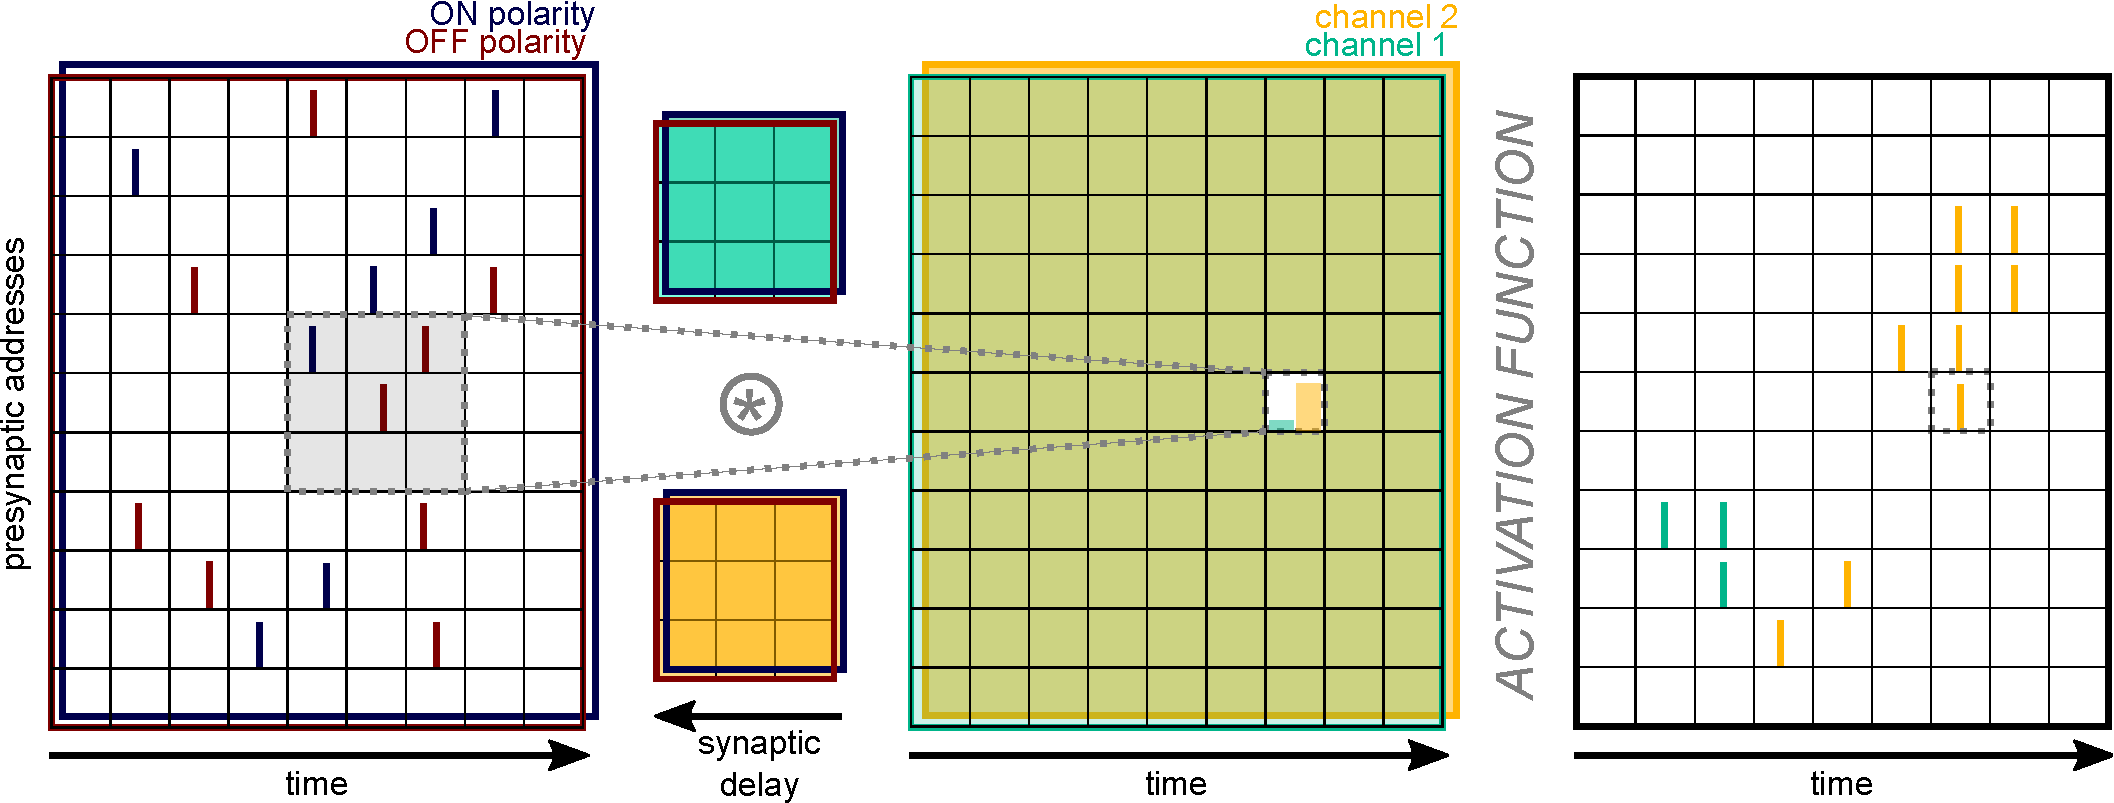
\includegraphics[width=\linewidth]{figures/HDSNN_conv.pdf}
    % 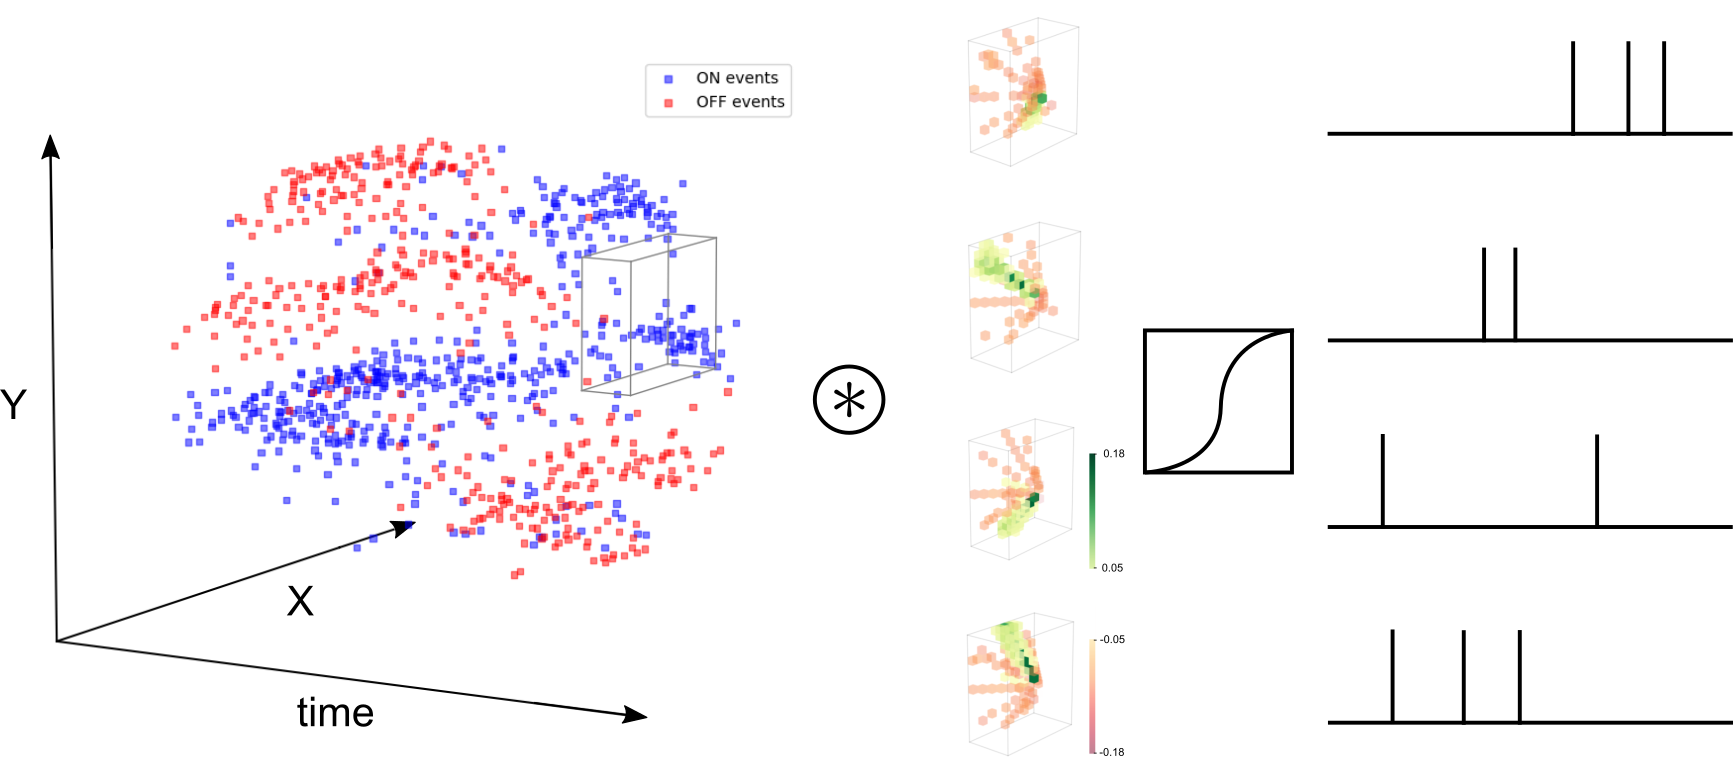
\includegraphics[width=\linewidth]{figures/HD-SNN.png}
    \caption{
    % \textbf{- HD-SNN illustration. From left to right:} A 3D representation of the event stream as output of the DVS. A 3D convolution is applied, on the dense representation of the input, along the $X$ and $Y$ spatial axes (defining the DVS pixel grid) and the temporal axis. There are as many kernels as the possible number of motion classes in the recording. For clarity, only $4$ kernels are illustrated and some weights are not represented in the voxel grid. For each voxel on the dense representation of the event stream as input, the output of the 3D convolution is processed by the non-linearity of the MLR model (i.e. softmax function). The output of the MLR gives a probability for each class, associated to a specific kernel, to emit an output event, or spike. With an appropriate spiking mechanism, here a winner-takes-all, we obtain, as output of the HD-SNN model, a new spike train with the different spikes associated to a specific motion class. }
    \textbf{Applying HD-SNN to the task of motion detection.} \textit{(Left)}~We plot here as a raster plot a 2D representation of the input event stream (showing ON spikes in red and OFF spikes in blue for each presynaptic address and time). A spatio-temporal convolution is applied to the dense representation of the input with $2$ distinct convolutional kernels (the green and orange kernels) that will define the output channels. The convolution is summed over the two polarities. If you have two axes $X$ and $Y$ to represent the presynaptic addresses as for the pixel grid of a DVS, you obtain a 3D convolution. We restrict the illustration to a 2D representation and to 2 possible classes (green and orange) that are associated with different motion directions. \textit{(Middle)}~For each position (address, time), one can compute the activation resulting from the convolution. The output of the convolution is processed by the nonlinearity of the MLR model (i.e., the softmax function). The output of the MLR gives a probability for each class associated with a particular kernel (colored bars in the highlighted pixel). \textit{(Right)}~By adding a spiking mechanism, here a winner-takes-all associated to a thresholding, we obtain as output of the HD-SNN model a new spike train with the different spikes associated to a specific motion class. Note that the position of the output spikes does not systematically correspond to the position of the input spikes but only when enough evidence is obtained.}
    \label{fig:model}
\end{figure}

\subsection{Supervised learning of the motion detection task}
%
Since the model is fully differentiable, we can now implement a supervised learning rule. This rule was implemented using the binary input events as inputs and the corresponding motion direction labels as the desired output. The loss function of the MLR model is the binary cross entropy at the output of the classification layer. The labels were defined at each time point as a one-hot encoding of the current motion in the channel corresponding to the current motion for all positions. Note that in this context, the label is known but the position is not, mainly due to the sparse spatial content of natural images. However, the supervised optimization of this MLR model will involve adjusting the weights of the kernels. As a result, the error is only propagated back to the spatial locations of these most active cells. This is reminiscent of previous methods that solve this problem using a winner-takes-all mechanism~\citep{masquelier_unsupervised_2007}, but is implicit in our formulation. Simulations are performed with the \note{PyTorch library using gradient descent with Adam (for $2^{12}$ movies and a learning rate of $10^{-5}$)}. We have shown in a previous work on a simplified task using synthetic textures that this type of learning algorithm can be assimilated to a Hebbian learning mechanism~\cite{grimaldi_robust_2022}.

Finally, the output of the MLR model is an event-based representation that predicts the probability of each motion at each position and time. Such an output provides a form of optical flow that can be exploited for non-rigid motion, but we have defined here, for simplicity, an evaluation method that applies to our full-field motion task. We have shown above that if different independent observations (here, the estimated motion at different spatial locations) are recognized as having a common cause (here, the rigid motion of the image), then an optimal estimate of the logit of this probability is the sum of the logits of the independent probabilities. Thus, by taking the mean logit of the probability of the output given by the model at all positions for any given time, we can calculate the probability of the output at this time. This allows one to calculate the accuracy (as the percentage of times the motion is accurately predicted). These calculations are performed on a different input data set than the one used in the training or validation steps. The complete code to reproduce the results of this paper is available at \url{https://github.com/SpikeAI/2023_GrimaldiPerrinet_HeterogeneousDelaySNN}. %
%
\section{Results}
\label{sec:results}
%%%-----------------------------------------------------------------
%: fig:kernels
%%%-----------------------------------------------------------------
\subsection{Kernels learned for motion detection}
%%%-----------------------------------------------------------------
\begin{figure*}[ht!]
    {\centering
    %\vspace{-3cm}
    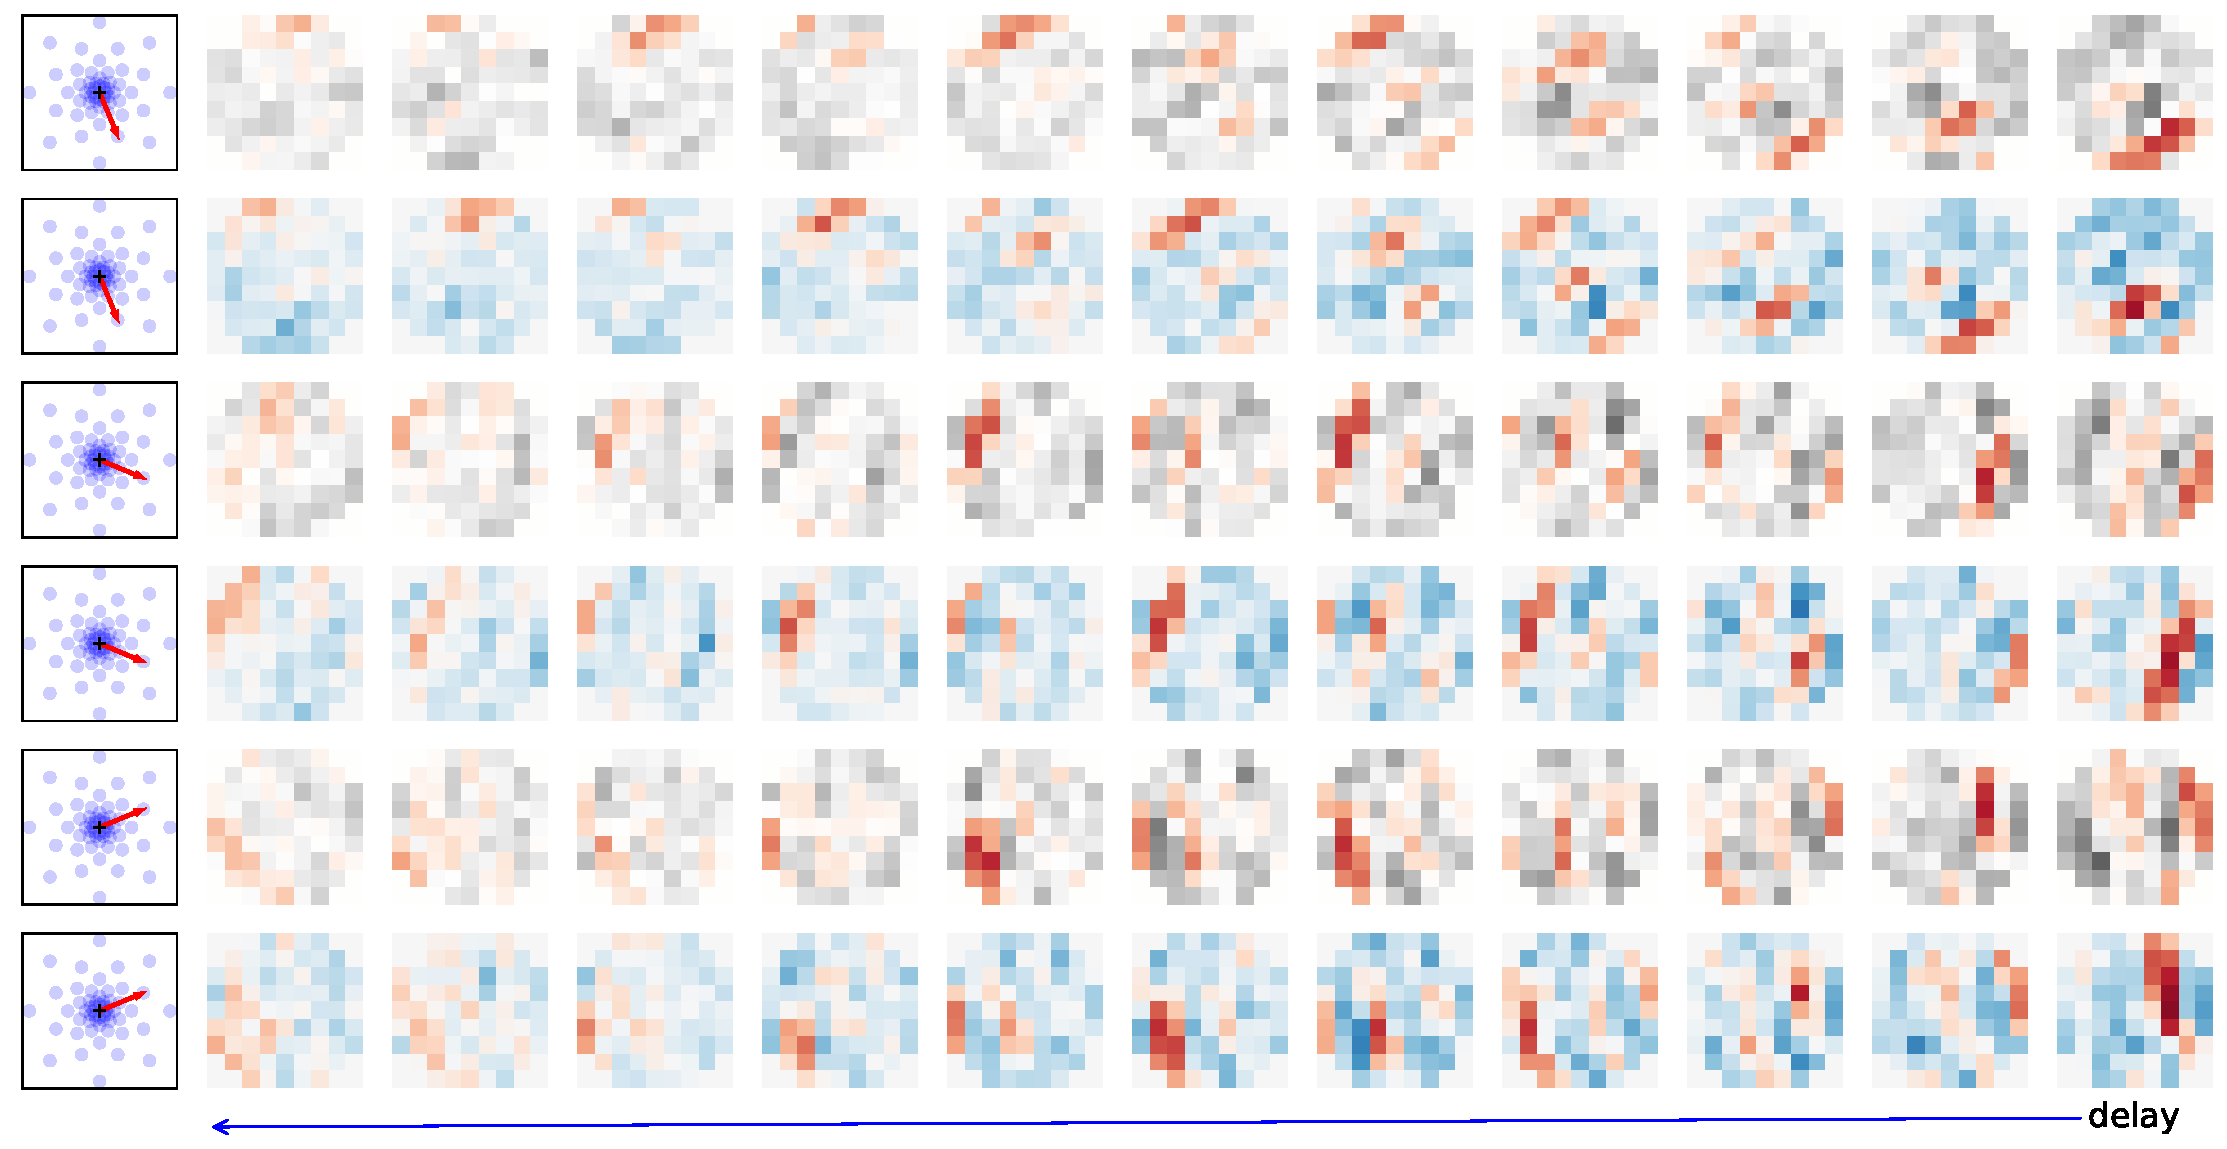
\includegraphics[width=\linewidth]{figures/motion_kernels.pdf}
    }
    %\vspace{-.5cm}
    \caption{
    	Representation of the weights for $8$ directions for one speed (among the $8 \times 3$ different kernels of the model) as learned on the dataset of naturalistic scenes. Directions are shown as red arrows on the left. The spatio-temporal kernels are represented as a sequence of images at different delays along the horizontal axis from the far right (delay of one step) to the left (delay of $12$ steps). Each image corresponds to the weights at a given delay, with excitatory and inhibitory weights in warm and cold colors, respectively. Due to the observed symmetry between the ON and OFF event streams, we observed that the kernels for the OFF polarities are very similar and are not shown here.	Different kernels are selective to the different motion directions and we observe a slight level of orientation selectivity perpendicular to the orientation. 
%      % These weights are associated to a specific delay on the \textit{delays} axis and to a presynaptic address defined on the two other axes. %	For the sake of clarity, the values in range $[-0.05, 0.05]$ are not shown.    One sees positive (excitatory) coefficients for the specific direction of motion but also negative (inhibitory) coefficients for other directions.
	}
    \label{fig:kernels}
\end{figure*} 
%
%
After training our model, we first analyze the weights learned for the different neurons (\seeFig{kernels}). 
We first observed a high dependence between the weights reaching the ON polarities and that reaching the OFF polarities. In particular, whenever a weight for a given position and delay is positive for one polarity, it will be negative in the other. This property comes from the way the events are generated and that the luminance can not at the same time increase and decrease. %ith the negative weights, one can observe an anti-selectivity for directions that do not correspond to the motion to which the kernel is selective to. 
We also observe that these cells show an orientation selectivity, similar to that observed in MT neurons~\citep{deangelis_functional_1999}. Interestingly, the relative organization of the receptive fields in quadrature of phase follows a push-pull organization predicted by~\citet{kremkow_push-pull_2016} to explain neurophysiological results observed after showing similar natural scenes with synthetic eye movements~\citep{baudot_animation_2013}. Focusing on the positive weights, a strong selectivity is observed along specific axes of motion for each of the different kernels. These directions can be easily associated to the direction of motion controlled in the natural images. For instance, the first kernel shows a strong selectivity to horizontal motion directions.
%
%This qualitative look at the 3D kernels allows the reader to infer for the $8$ different motion directions used to generate our synthetic event streams.

If one focuses on the interpretation of these kernels in terms of spatio-temporal motifs embedded in the event stream, it can lead to interesting outcomes. In~\citep{grimaldi_robust_2022}, a link between event-based MLR training and Hebbian learning is drawn, allowing to say that the present model will learn its weights according to a presynaptic activity associated to the different motion directions. Each neuron becomes selective to a specific motion direction through the learning of an associated prototypical spatio-temporal spike motif. Each voxel in the 3D kernels defines a specific timestamp and a specific address. Consequently, our model is able to detect precise spatio-temporal motifs embedded in the spike train and associated to the different motion directions. The cone shape for the positive weights distribution highlights a loss of precision for longer delays, i.e. events away in the past. For the directions not coherent to the class of a training sample, an anti-Hebbian learning is also observed through the negative weights in the kernels of Fig.~\ref{fig:kernels}. 

%
% \note{kernel size has to be adapted to the characteristics of motion see Samonds %~\citep{samonds}
% say that we have tested }
% \note{tester la meme expe faite par baudot et modelisée par kremkow en montrant des raster plots du modele avec NI versus Gratings }

%%%-----------------------------------------------------------------
%
\subsection{Testing with natural-like textures}
%%%-----------------------------------------------------------------
To test our model, we will quantify its ability to categorize different motions, that is on event streams for which the ground truth motion is known at every instant in time. Before applying the model on natural images, we will first test the model on simpler, parameterized stimuli. In that order, we use a set of synthetic visual stimuli, \textit{Motion Clouds}~\citep{leon_motion_2012} which are natural-like random textures for which we can control for velocity, among other parameters (\seeFig{motion_clouds})~\citep{vacher_bayesian_2018}. In particular, we will set the spatial size and duration similarly to the motion task defined above. This procedure defines a set of textures with different spatial properties and different motions $\va{v}_k$ with  $1 \le k \le \Nclass$ and $\Nclass=8$ defined by a constant speed and linearly spaced directions $
\speed_\kernelind = 
  ( 
    \speed \cdot \cos(2\pi\cdot \frac{\kernelind}{\Nspeed}),
    \speed \cdot \sin(2\pi\cdot \frac{\kernelind}{\Nspeed})
  )
$.
For any given velocity, we also varied the parameters of the textures, such as the mean and variance of the orientation or spatial frequency content to provide with some naturalistic variability. This method provides a rich dataset of textured movies for which we know the ground truth for motion.
%%%-----------------------------------------------------------------
%: fig:motion_clouds
%%%-----------------------------------------------------------------
\begin{figure}%[h!]
    \centering
    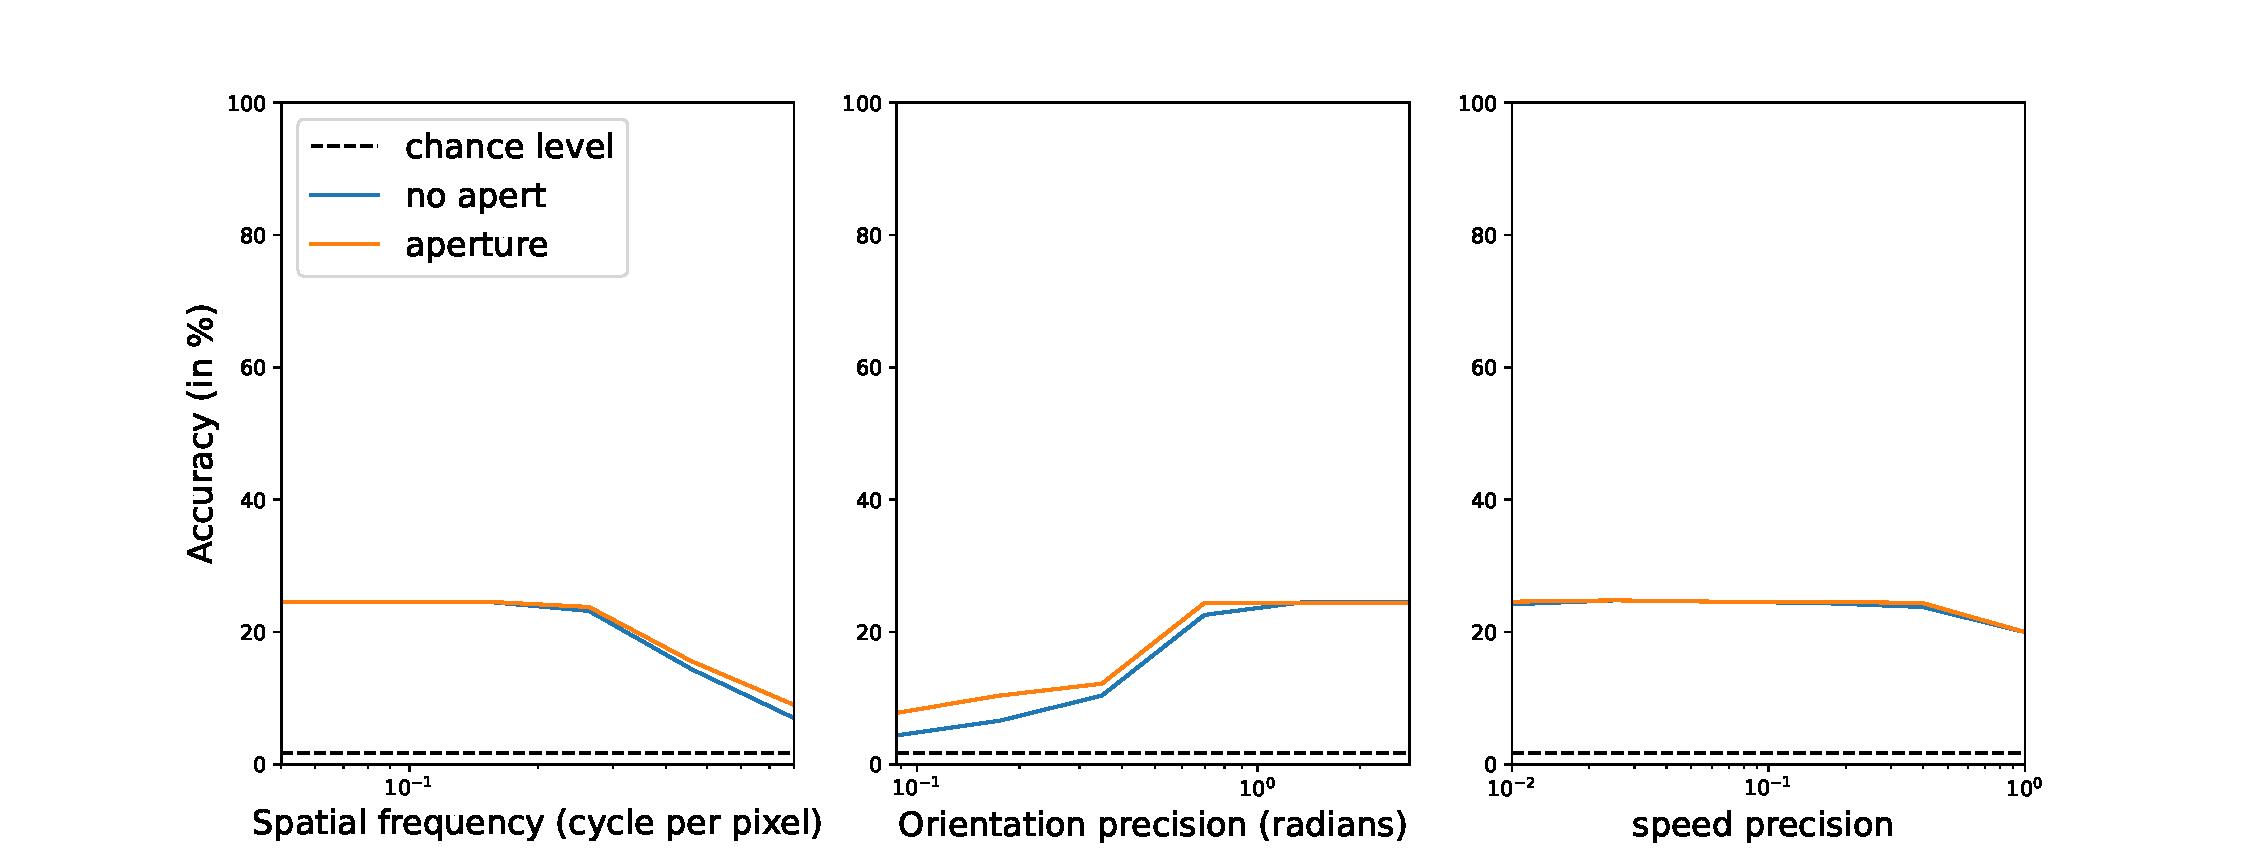
\includegraphics[width=0.99\linewidth]{figures/motion_clouds.pdf} %
    \caption{{\bf Role of stimulus parameters in the motion detection accuracy.} Accuracy as a function of (from left to right) the mean spatial frequency, the bandwidth in orientation (from a grating-like (left) to isotropic textures (right)), the bandwidth in spatial frequency, the bandwidth in speed, from a rigid motion (left) to independent frames (right). Note that these accuracy is computed both in the case where orientation of the synthetic texture is necessarily perpendicular to the motion ('no aperture' condition) or in the arbitrary case where orientation is independent of direction ('aperture').}
    \label{fig:motion_clouds}
\end{figure}
%%%-----------------------------------------------------------------

We plot here main axis of interests. First, as we change the mean spatial frequency of the texture, we observe a monotonous decrease in accuracy. This comes as a similar trend as that observed in the primary visual areas~\citep{priebe_tuning_2006}. %\note{we should really do something more serious here...} 
Notably, the accuracy is better for a large spatial frequency bandwidth (which qualitatively resemble a more textured stimulus) than for a grating-like stimulation, reminiscent to the behavioral response of humans' eye movements to such stimuli~\citep{simoncini_more_2012}. Interestingly, we also see a modulation of accuracy as a function of orientation bandwidth. When the stimulus is grating-like and that the orientation is arbitrary with respect to the direction of motion, the system is faced with the aperture problem and see a decrease of accuracy. This is not the case for isotropic stimuli or when the orientation is perpendicular to the direction of motion. Finally, we manipulated the amount of change between two successive frames, similar to a temperature parameter. This shows a progressive decrease in accuracy, similar to that observed in the amplitude of humans' eye movements~\citep{mansour_pour_speed_2018} but also that accuracy is low for a rigid motion which lacks variability.
%
\subsection{Accuracy efficiency trade-off}% for the motion detection task}
%%%-----------------------------------------------------------------
Once our MLR is trained, we obtain spatio-temporal kernels corresponding to the weights associated to the heterogeneous delays of our layer of spiking neurons and which may be used for detection. We observed that the distribution of the kernels' weights is sparse, with most values near zero. As shown in the formalization of our event-based model, the computational cost of our model if implemented on a neuromorphic chip would be dominated by the number of spikes times the number of synapses. Indeed, the computations are dominated by the convolution operation. In a dense setting, this corresponds for all voxels in the output to a sum over all voxels in the inputs for all weights in the kernel. If the support of information is sparse, then computations can be performed only on those events. Also, if we set some weights of the kernels to zero, then the sum can be skipped for those addresses. Knowing the sparseness of the input, the total number of computations thus scales with the number of nonzero synaptic weights. 

To assess the robustness of the classification as a function of the computational load, we will prune the weights in $\{\synapse_\ranksyn\}_{\ranksyn \in [0,\Nsyn)}$ that are below a defined threshold. In Fig.~\ref{fig:accuracy}, we plot the classification accuracy as a function of the relative number of computations, or active weights, per decision for each neuron of the layer. As a comparison and to account for the gain in performance by using heterogeneous delays, we provide the accuracy obtained with a MLR model using 2D time surface (in red) as in~\citep{grimaldi_robust_2022}. This latter method is based on delays from the last recorded events and uses fewer computations (in our case $15\times15$) than the dense 3D kernels without any pruning ($15\times15\times8$). While less computations are needed, the classification performance obtained for the model using time surfaces is similar to our method using all the weights of the kernels.

By pruning weights, we observe that the evolution of accuracy as a function of the log percentage of active weights fits well a sigmoid curve. Half-saturation level is reached at about $3.5\times 10^{-3}\%$ of active weights, corresponding in our setting to a total amount of $6$ computations per decision. Compared to the full kernels, the accuracy of our method is maintained to its top performances when dividing the number of computations by a factor up to about $200$. In this case, the number of computations is greatly reduced compared to~\citep{grimaldi_robust_2022}, thus demonstrating the efficiency of the presented method. 
%
%%%-----------------------------------------------------------------
%: fig:accuracy
%%%-----------------------------------------------------------------
\begin{figure}%[h!]
    \centering
    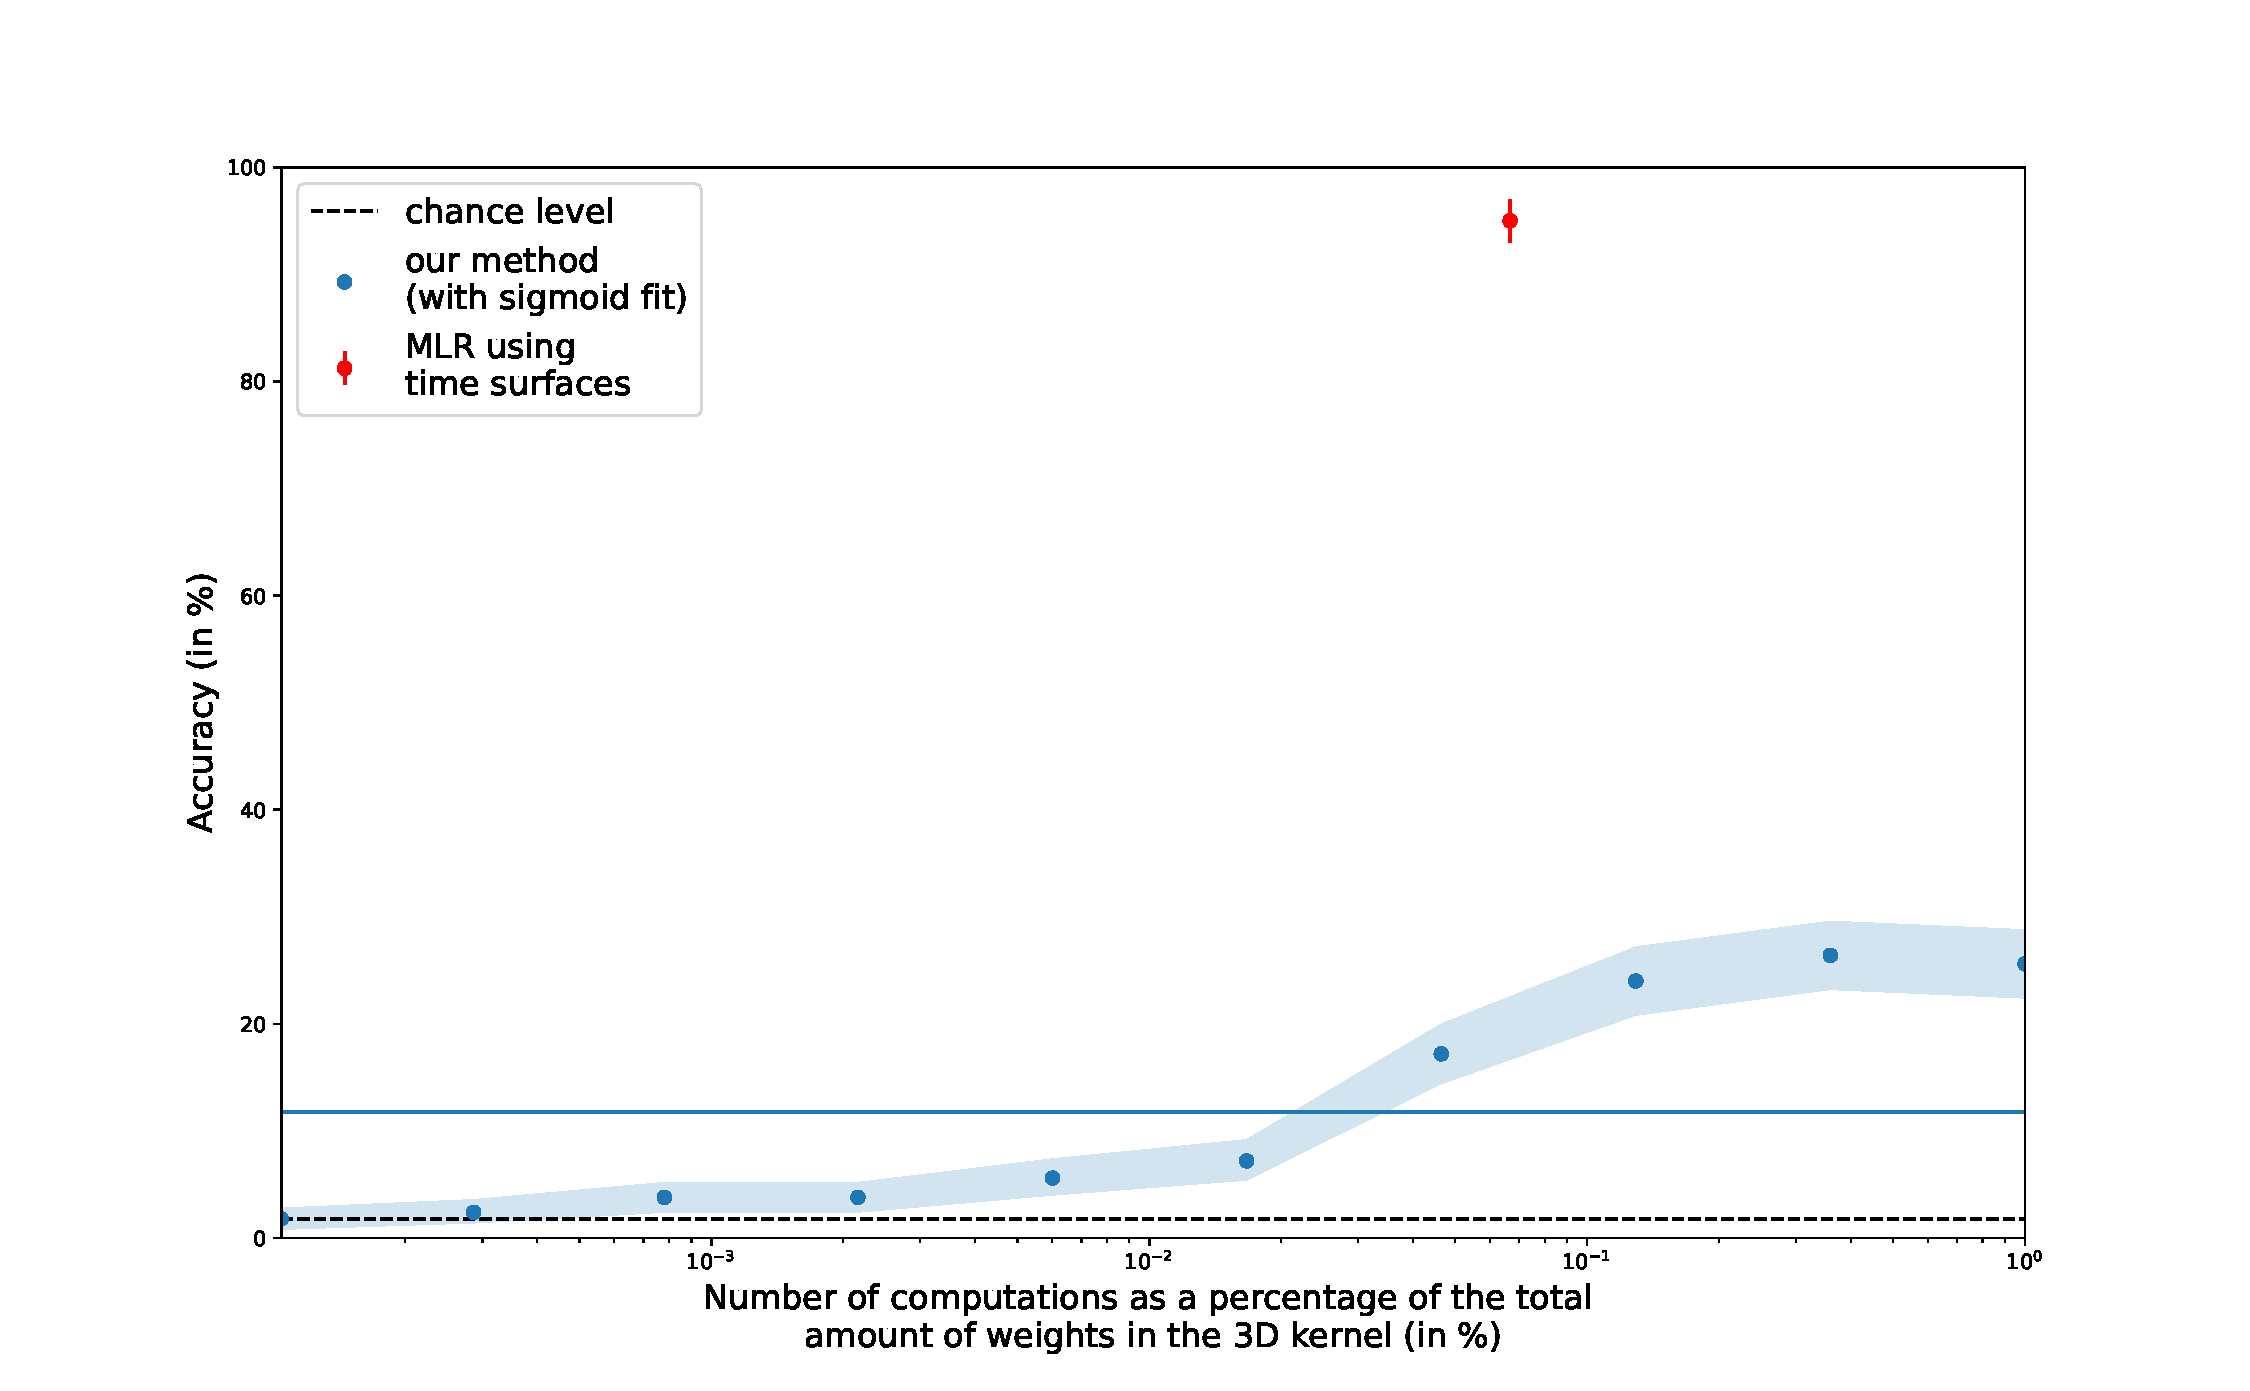
\includegraphics[width=0.95\linewidth]{figures/quant_accuracy.pdf}
    \caption{Accuracy as a function of computational load for the HD-SNN model (blue dots) with error bars indicating the 5\% - 95\% quantiles and a sigmoid fit (blue line). The relative computational load (on a logarithmic axis) is controlled by changing the percentage of nonzero weights relative to the dense convolution kernel. As we prune the coefficients, we observe a stable accuracy value, with a drop observed at about 25 times fewer computations.}
    \label{fig:accuracy}
\end{figure}
%
\section{Discussion}
%%%-----------------------------------------------------------------
In this paper, we have introduced a generic SNN with heterogeneous delays and shown how it compares favorably to a state-of-the-art event-based classification algorithm for a visual motion detection task. The learned model shares a number of similarities with neurobiological anatomical observations, as well as with behavioral results. The event-based computations of our method can be drastically reduced by pruning synapses, while maintaining top classification performance. This shows that we can take advantage of the precise timing of spikes to improve the performance of neural computations.
%
\subsection{Synthesis and main contributions}
%%%-----------------------------------------------------------------
The HD-SNN model that has been trained and evaluated on a complex motion detection task. The model has been defined to provide optimal detection of event-driven spatio-temporal motifs. We have shown that the model, when trained on a dataset of natural images with realistic eye movements, learns kernels similar to those found in the early visual cortex~\cite{kremkow_push-pull_2016}. %We then demonstrated that the model shows similarities to biological responses.
We have evaluated the computational cost of this model when implemented in a setting similar to event-based hardware. We show that the use of heterogeneous delays may be an efficient computational solution for future neuromorphic hardware, but also a key to understanding why spikes are a universal component of neural information processing.

We would like to highlight a few innovations in the contributions that are presented in this paper. First, whereas~\citep{ghosh_spatiotemporal_2019,yu_stsc-snn_2022} use a correlation-based heuristic, which we observed to be less efficient, the generic heterogeneous model is formalized from first principles for optimal detection of the event-based spatio-temporal motifs. Moreover, in comparison to a representation with time surfaces, the weights are explicable as they directly inform on the logit (inverse sigmoid of the probability) of detection of each spatio-temporal spike motif. Another novelty is that the model learns the weights and the delays simultaneously. For example, the polychronization model~\citep{izhikevich_polychronization_2006} learns only the weights using STDP, while the delays are randomly drawn and their values are frozen during learning. In addition, the model is evaluated on a realistic task, while models such as the tempotron are tested on simplified toy problems~\citep{gutig_tempotron_2006}. Another major contribution is to provide a model that is suitable for learning any kind of spatio-temporal spiking motifs and that can be trained in a supervised manner by providing a dataset of supervision pairs. Instead of relying on a careful description of the physical rules governing a task, e.g. the luminance conservation principle for motion detection~\citep{benosman_asynchronous_2012, dardelet_event-by-event_2021}, this allows a more flexible definition of the model using this properly labelled dataset.
%
\subsection{Main limits}
%%%-----------------------------------------------------------------
We have identified a number of limitations of our model, which we will now discuss in detail. First, the entire framework is based on a discrete binning of time, which is not compatible with the continuous nature of biological time. We used this binning to efficiently implement the framework on conventional hardware, especially GPUs, to be able to use fast three-dimensional convolutions. We have tested the effect of the width of the time bin and shown that it has essentially no effect on the results presented in this paper. This is consistent with the relative robustness of other event-based frameworks such as HOTS~\citep{lagorce_hots_2017}, where accuracy was unaffected when the input spikes were subjected to noisy perturbations up to $1~\ms$~\citep{grimaldi_robust_2022}. This suggests the possibility of analytically including a precision term in the temporal value of the input spikes. This mechanism may be implemented by the filtering implemented by the synaptic time constant of about $5~\ms$. Furthermore, it is possible to circumvent the need for time discretization by the use of a purely event-based scheme. In fact, it is not necessary to compute the voltage traces between two spikes~\citep{hanuschkin_general_2010}. Thus, it is possible to define a purely event-based framework. Such an architecture could provide promising computational speedups. % \note{pourrait parler du poster bernstein? de nadafian?}

A further limitation is that the model is purely feed-forward. Thus, the spikes generated by the postsynaptic neurons are based solely on information contained in the classical receptive field. However, it is well known that neurons in the same layer can interact with each other using lateral interactions, for example in V1, and that this can be the basis for computational principles~\citep{chavane_revisiting_2022}. For example, the combination of neighboring orientations may contribute to image categorization~\citep{perrinet_edge_2015}. Furthermore, neural information is modulated by feedback information, e.g. to distinguish a figure from its background~\citep{roelfsema_early_2016}. Feedback has been shown to be essential for building realistic models of primary visual areas~\citep{boutin_sparse_2020, boutin_effect_2020}, especially to explain non-linear mechanisms~\citep{boutin_pooling_2022}. Currently, mainly due to our use of convolutions, it is not possible to implement these recurrent connections in our implementation (lateral or feedback). However, by inserting new spikes into the list of spikes reaching presynaptic addresses, the generic model is able to incorporate them. While theoretically possible, this needs to be properly adjusted in practice so that these recurrent connections do not amplify neuronal activity outside a homeostatic state (by extinction or explosion).
% \note{ dire que la prédiction permet de faire de la prediction et que ça explique les résultats de leBec}%~\citep{perrinet_motion-based_2012}

Such recurrent activity would be essential for the implementation of predictive or anticipatory processes. This is essential in a neural system because it contains several different delays that require temporal alignment~\citep{hogendoorn_predictive_2019}. This has been modeled before to explain, for example, the flash-lag illusion~\citep{khoei_flash-lag_2017}. %\note{Say that this could be implemented by properly setting the timing of the label} 
As mentioned previously, this could be implemented using generalized coordinates (i.e., variables such as position complemented by velocity, acceleration, jerk,~\ldots), and ``neurobiologically, using delay operators just means changing synaptic connection strengths to take different mixtures of generalized sensations and their prediction errors''~\citep{perrinet_active_2014}. Our proposed model using heterogeneous delays provides an alternative and elegant implementation solution to this problem.
%
\subsection{Perspectives}
%%%-----------------------------------------------------------------
% \note{la tache ne met pas en avant les capacites des motifs hetero synaptiques =trop simple et peut se faire en HOTS}
In defining our task, we emphasized that the generation of events depends on the spatial gradient in each image. This gradient has both horizontal and vertical dimensions, and its maxima are generally orientation dependent. Taken together, these oriented edges form the contours of visual objects in the scene~\citep{koenderink_representation_1987}. Thus, there is an interdependence between the information about motion and the information about orientation within the event stream. It would be crucial to investigate this dependency further. This could be initiated by training the model on a dataset with labels that provide local orientation. %\note{we can say that we tried it and that it works well}. 
Exploring this dependence will allow us to dissociate these two forms of visual information and enable us to integrate them. In particular, it will allow us to consider that the definition of motion is more accurate perpendicular to an oriented contour (aka the aperture problem). Thus, it will allow us to implement recurrent prediction rules, such as those identified to dissociate this problem~\citep{perrinet_motion-based_2012}.

The model is trained on a low-level local motion detection task, and one might wonder if it could be trained on higher-level tasks. An example of such a task would be the estimation of depth in the visual scene. There are several sources of information for depth estimation, such as binocular disparity or changes in texture or shading, but in our case motion parallax would be the most important cue~\citep{rogers_motion_1979}. This is because objects that are close to an observer will move relatively faster on the retina than an object that is far away, and also because visual occlusions are dependent on the depth order. Using this information, it is possible to segment objects and estimate their depth~\citep{yoonessi_contribution_2011}. However, this would require the computation of the optical flow first, i.e., the extension of the framework described here for a rigid full-field motion to a more general one where the motion may vary in the visual field. A possible implementation is therefore to add a new layer to our model, analogous to the hierarchical organization highlighted in the visual cortex. This is theoretically possible by using the output of our model (which estimates velocity in retinotopic space) as input to a new layer of neurons that would estimate velocity in the visual field, including the depth dimension in the output supervision labels. This could have direct and important applications, e.g. in autonomous driving to detect obstacles in a fast and robust way. Another extension would be to actively generate sensor motion (physical or virtual) to obtain better depth estimates, especially to disambiguate uncertain estimates~\citep{nawrot_eye_2003}.

In conclusion, the model that we have presented provides a way to process event-based signals in an efficient manner. We have shown that we can train the model semi-supervised, knowing \emph{what} output label, but not \emph{when} it occurs. Another perspective would be to extend the model to a fully self-supervised learning paradigm, i.e., without any labeled data~\citep{barlow_unsupervised_1989}. This type of learning is thought to be prevalent in the central nervous system and, assuming the signal is sparse~\citep{olshausen_emergence_1996}, one could extend these Hebbian sparse learning schemes to spikes~\citep{perrinet_emergence_2004, masquelier_competitive_2009}. We expect that this would be particularly useful for exploring neurobiological data. Indeed, there is a large literature showing that brain dynamics often organize into stereotyped sequences, such as synfire chains~\citep{ikegaya_synfire_2004}, packets~\citep{luczak_sequential_2007}, or hippocampal sequences~\citep{pastalkova_internally_2008, villette_internally_2015}. These patterns are stereotyped and robust, as they can be activated in the same pattern from day to day~\citep{haimerl_internal_2019}. In contrast to conventional methods of processing neurobiological data, such an event-based model would be able to answer key questions about the representation of information in neurobiological data, and it would open up possibilities in the field of computational neuroscience. Furthermore, it would open up possibilities in the field of machine learning, especially in computer vision, to address current key concerns such as robustness to attacks, scalability, interpretability, or energy consumption.
%
%%%%%%%%%%%%%%%%%%%%%%%%
\backmatter
%
\bmhead{Acknowledgments}
%
\Acknowledgments
%
%%%%%%%%%%%%%%%%%%%%%%%%

\section*{Statements and Declarations}

\paragraph{Funding}

\Funding %

\paragraph{Conflict of interest}
Not applicable.

\paragraph{Ethics approval}
Not applicable.

\paragraph{Consent to participate}
Not applicable.

\paragraph{Consent for publication}
Not applicable.

\paragraph{Availability of data and materials}
Not applicable.

\paragraph{Code availability}
%
\DataAvailability
%   
\paragraph{Authors' contributions}
%
Both authors contributed to the conceptualization and methodology design of the study, to the project's coordination and administration. Laurent Perrinet carried out the funding acquisition and supervision. Formal analysis and investigation were performed by both authors. Results visualization and presentation were realized by both authors. The manuscript was written by both authors. Both authors have read and approved the final manuscript.
%%%%%%%%%%%%%%%%%%%%%%%%
\bibliographystyle{apalike}
\bibliography{FastMotionDetection}
\end{document}
%%%%%%%%%%%%%%%%%%%%%%%%